% !TeX spellcheck = cs_CZ
\documentclass[czech,master,dept460,male,csharp,cpdeclaration]{diploma}

\usepackage[autostyle=true,czech=quotes]{csquotes} % korektni sazba uvozovek, podpora pro balik biblatex
\usepackage[backend=bibtex, style=iso-numeric, alldates=iso]{biblatex} % bibliografie
\usepackage{dcolumn} % sloupce tabulky s ciselnymi hodnotami
\usepackage{subfig} % makra pro "podobrazky" a "podtabulky"
\usepackage{rotating}

\usepackage{geometry}
\usepackage{listings}
\usepackage{tikz}
\usepackage{pgfplots}

\usepackage{xcolor}
\usepackage{listings}

%\usepackage{mathtools} %- blokuje list obrázků a tabulek

\ThesisAuthor{Bc. Jan Jedlička}

\ThesisSupervisor{prof. Ing. Michal Krátký, Ph.D.}

\CzechThesisTitle{Key-value databázové systémy}

\EnglishThesisTitle{Key-value database systems}

\SubmissionYear{2024}

\ThesisAssignmentFileName{ThesisSpecification_JED0050_vsboee2302B326.pdf}

\Acknowledgement{Na tomto místě bych chtěl poděkovat vedoucímu této práce prof. Ing. Michalovi Krátkému, Ph.D., za poskytnutí užitečných rad a pomoci vedením práce.}

\CzechAbstract{Cílem diplomové práce je popsat Key-value DBS, ukázat výhody a nevýhody těchto systémů a představit některé významné zástupce. První část práce je zaměřena nejen na obecný popis Key-value DBS, ale i na podrobnější specifikace vybraných DBS a jejich vzájemné porovnání. Součástí práce je zmapování existujících testů DBS a následný výběr a zprovoznění testovacího prostředí pro testování těchto systémů a porovnání s ostatními DBS. Práce popisuje dva významné představitele testovacích prostředí DBS, YCSB a TPC. S prostředím YCSB se v práci následně pracuje a testují se v něm čtyři vybrané Key-value DBS: Redis, Aerospike, Riak KV a Memcached. Veškeré testy jsou spouštěny pomocí skriptů, které spustí a nastaví DBS v prostředí Docker. Připravené DBS jsou následně naplněny daty a otestovány za pomoci prostředí YCSB. Práce je zakončena reprezentací hodnot naměřených při testování, vzájemným porovnáním pomocí grafů a vyhodnocením výsledků těchto testů.}

\CzechKeywords{DBS; NoSQL; Key-value DBS; Benchmarking; YCSB; TPC; Redis; Riak KV; Aerospike; Memcached}

\EnglishAbstract{The aim of this thesis is to describe Key-value DBS, to show the advantages and disadvantages of these systems and to introduce some important representatives. The first part of the thesis focuses not only on a general description of Key-value DBSs, but also on more detailed specifications of selected DBSs and their comparison with each other. The work includes a mapping of existing DBSs and then the selection and operationalization of a testbed for testing these systems and comparing them with other DBSs. The thesis describes two prominent representatives of DBS test environments, YCSB and TPC. The YCSB environment is then used in the thesis to test four selected key-value DBSs: Redis, Aerospike, Riak KV and Memcached. All tests are run using scripts that start and set up the DBS in the Docker environment. The prepared DBSs are then populated with data and tested using the YCSB environment. The paper concludes by representing the values measured during testing, comparing them with each other using graphs and evaluating the results of these tests.}

\EnglishKeywords{DBS; NoSQL; Key-value DBS; Benchmarking; YCSB; TPC; Redis; Riak KV; Aerospike; Memcached}

\AddAcronym{DBS}{Databáze}
\AddAcronym{NoSQL}{Not only Structured Query Language}
\AddAcronym{Key-value DBS}{Klíč-hodnota DBS}
\AddAcronym{KDBS}{Key-value DBS}
\AddAcronym{RDBS}{Relační DBS}
\AddAcronym{JSON}{JavaScript Object Notation}
\AddAcronym{TTL}{Time to live}
\AddAcronym{TPC}{Transaction Processing Performance Council}
\AddAcronym{YCSB}{Yahoo! Cloud Serving Benchmark}
\AddAcronym{Kiloops}{Tisíce operací}

\addbibresource{citace.bib}

\begin{document}
	
	\MakeTitlePages
	
	\listoffigures
	\listoftables
	
	\chapter{Úvod}
	
	Key-value (neboli Klíč-hodnota) databázové systémy~\cite{amaz-key-value-db, ytb-nosql-db}, dále jen zkráceně KDBS, jsou jedním z paradigmat pro úložiště dat. Databáze je navržena pro rychlý přístup k datům a uživatelsky snadnou práci. Pro manipulaci s daty se zpravidla používá několik příkazů pro vložení, získání, aktualizaci a odstranění hodnot na základě klíčů. V KDBS se hodnota ukládá k danému klíči, přičemž klíč může být například "jmeno\_uzivatele", a hodnota může být "Jan Novák".
	
	KDBS fungují odlišně oproti tradičním relačním databázovým systémům. Datový model RDBS je relační~\cite{rdbs}, což znamená, že data jsou organizována do tabulek, kde každá tabulka představuje jednu relaci~\cite{relace} a každý záznam v tabulce odpovídá jednomu řádku. Každá tabulka obsahuje sloupce, které předem pevně definují datové typy záznamů. Jedním ze sloupců je primární klíč, který jednoznačně identifikuje každý záznam. Tento relační model poskytuje strukturovaný a systematický přístup k ukládání a manipulaci s daty, což usnadňuje organizaci a vyhledávání informací. Díky definované struktuře záznamů může RDBS provádět řadu optimalizací, jako je například přidávání vlastních indexů nebo plánování a optimalizace dotazů~\cite{rdbs-optimalizace}. Například pokud chceme do RDBS ukládat záznamy obsahující uživatele, musí mít každý záznam stejnou strukturu. Takže uživatel musí obsahovat všechny povinné atributy, jako jsou jméno a příjmení, a dodržet jejich předem stanovený datový typ a velikost, například počet číslic v telefonním čísle. Pokud by záznam obsahoval nějaké atributy navíc, například informaci o tom, zda je uživatel nemocný, nebo by jejich datový typ neodpovídal očekávanému, je zapotřebí upravit i tabulku, do které záznam vkládáme, a také záznamy, které se již v této tabulce nachází.
	
	Na druhou stranu KDBS mohou mít pro každý klíč různě definované hodnoty, které mohou zahrnovat kolekce dat s odlišnými velikostmi. Tato vlastnost nabízí KDBS flexibilitu a možnost přiblížení se k objektově orientovanému programování. Například do KDBS s klíči jako ID uživatele a hodnotami reprezentujícími záznamy různých uživatelů můžeme ukládat JSON objekty. Tyto objekty reprezentují uživatele, kteří jsou definováni odlišnými, na sobě nezávislými třídami s různým počtem a datovým typem atributů, bez společného rodiče. Dále tyto databáze dosahují horizontální až lineární škálovatelnosti (viz kapitola~\ref{scaling-dbs}). Protože KDBS nevyžaduje pevně nastavené datové typy hodnot, jako je tomu u relační databáze, tak KDBS může vyžadovat méně paměti k uložení stejných dat~\cite{kdbs-memory}, což vede k nárůstu výkonu v určitých případech.
	
	Databáze se schématem~\cite{schemaless-vs-schema} (schema-on-write) vyžadují definici datového schématu před tím, než jsou data uložena. To znamená, že musíte předem definovat strukturu dat včetně typů dat, a poté můžete data vložit do DBS. Na druhou stranu databáze bez schématu (schema-on-read, schema-less) umožňují ukládat data bez předchozí definice datového schématu. Schéma je definováno až v okamžiku, kdy data čtete z DBS. To umožňuje pružnější přístup k ukládání a zpracování dat, ale může vést k menší kontrole nad strukturou dat a k možným problémům s konzistencí dat.
	
	Výkon a nedostatečná standardizace omezovaly KDBS pouze na specializovaná využití, ale díky rychlému přechodu na cloud computing, dochází v posledních letech k nárůstu popularity NoSQL databázových systémů, zatímco popularita RDBS je víceméně stejná~\cite{dbranking-trend-by-model}. Dle výzkumu z roku 2019~\cite{scalegrid-sql-vs-nosql} byly RDBS využívány v 60,48 \% případů napříč všemi databázovými systémy, zatímco NoSQL DBS pak zastávaly zbylých 39,52 \%. Často se však pro využití výhod různých druhů DBS využívá kombinace RDBS a NoSQL DBS. Tato kombinace je proto využívána v 75,6 \% případů. Čistě využívané RDBS poté zabírají 16,6 \% a NoSQL DBS 9,8 \%. 
	
	Webová stránka DB-Engines~\cite{dbranking-web-index} porovnává DBS na základě popularity. Bodové skóre popularity je spočítáno na základě počtu zmínek na webových stránkách, frekvenci diskuzí na technických fórech, pracovních nabídek a poptávek, relevance DBS na sociálních sítích, počtu profilů na profesních sociálních sítích zmiňujících danou DBS a obecného zájmu o DBS~\cite{dbranking-ranking-definition}. Při sledování trendu DBS od roku 2013 do současnosti~\cite{dbranking-trend-by-dbs} (viz graf~\ref{graf-dbranking-trend-dbs}) dochází k výraznému nárůstu hodnocení popularity NoSQL DBS, konkrétně KDBS Redis~\cite{redis} stoupla od roku 2013 z 25,973 bodů na 156,441 bodů, došlo tedy k nárůstu popularity o 502,68 \%. Pro RDBS Oracle~\cite{oracle-index} došlo naopak k poklesu popularity z 1559,332 bodů na 1234,269 bodů, pokles činí 20,85 \%. Trend změny hodnot popularity~\cite{dbranking-trend-by-model} (viz graf~\ref{graf-dbranking-trend-model}) pro RDBS obecně od roku 2013 se příliš nemění a dochází k poklesu v maximálně jednotkách bodů každý měníc, KDBS naopak znatelně stoupaly se svým hodnocením do konce roku 2022 a aktuálně dochází k poklesu popularity v řádu několika jednotek bodů každý měsíc.
	
	Například databázový systém Redis je v současnosti jedním z deseti nejlépe hodnocených~\cite{db-engineers-ranking} databázových systémů napříč relačními i NoSQL databázovými systémy. V žebříčku porovnání téměř 70 čistě KDBS~\cite{db-engineers-ranking-kdbs}, je Redis na prvním místě, za ním následují Amazon DynamoDB~\cite{dynamodb}, společně s Microsoft Azure Cosmos DB~\cite{azure-cosmos-db} a Memcached~\cite{memcached}.
	
	Cílem práce je prostudovat a podrobně popsat problematiku KDBS. Práce se zaměří na vysvětlení tohoto konceptu a identifikaci klíčových rozdílů mezi jednotlivými KDBS. Jednou z hlavních úloh práce je zmínit a detailně popsat některé z nejznámějších a nejčastěji využívaných databázových systémů v tomto odvětví. Tyto DBS budou vzájemně porovnány s důrazem na jejich vlastnosti, výhody a nevýhody. Dalším úkolem práce je příprava a zprovoznění testovacího prostředí, které umožní měření propustnosti a odezvy na dotazy těchto vybraných KDBS. Návrh a implementace testovacího prostředí zahrnuje konfiguraci prostředí a zprovoznění instancí databázových systémů, ať už lokálně nebo v cloudovém prostředí. Následně budou vybrané DBS podrobeny testování a budou měřeny jejich propustnosti a latence v reálném provozu. Naměřené hodnoty budou prezentovány a analyzovány s cílem porovnat chování jednotlivých DBS v různých scénářích. Konečné výsledky budou porovnány, což umožní vyvodit závěry o tom, jak se jednotlivé DBS osvědčily v praxi při manipulaci s daty.
	
	Struktura práce je následující. První část práce (viz kapitola \ref{chapter:no-sql-ky-sys}) se zaměřuje na detailní představení několika klíčových KDBS (např. Redis, Riak KV, Aerospike). Každá z těchto DBS je popsána, a to včetně analýzy jejich charakteristických vlastností. V závěru této části je provedeno srovnání jednotlivých databází na základě jejich vlastností, například škálovatelnost, dotazovací jazyk a odezva.
	
	Kapitola 3 (viz kapitola \ref{chapter:3-test_environment}) obsahuje popis a využitelnost testovacích prostředí databázových systémů. V kapitole jsou uvedena dvě existující testovací prostředí TPC~\cite{tpc} a YCSB~\cite{ycsb}. Testovací prostředí TPC je využíváno především pro relační databázové systémy, zatímco prostředí YCSB je připraveno a vyvíjeno zejména pro NoSQL DBS.
	
	Kapitola 4 (viz kapitola \ref{chapter:4-test_results}) je věnována testování a vyhodnocení výsledků čtyř vybraných KDBS (Redis~\cite{redis}, Riak KV~\cite{riak}, Aerospike~\cite{aerospike} a Memcached~\cite{memcached}). Tyto DBS byly vybrány pro analýzu z důvodu své relevance podle internetových žebříčků~\cite{db-engineers-ranking, predictiveanalyticstoday}. Kapitola popisuje stroj, na kterém se KDBS testovaly, a potřebnou přípravu zvoleného testovacího prostředí YCSB a databází v Dockeru~\cite{docker}. Konkrétně se zde popisují konfigurace jednotlivých testů, kroky pro úspěšné spuštění testů a samotné otestování. Kapitola je zakončena prezentací výsledků naměřených hodnot při testování a vzájemným porovnáním výsledků jednotlivých KDBS. 
	
	V závěru práce, kapitole 5 (viz kapitola \ref{chapter:5-diploma_results}), jsou vyhodnoceny výsledky srovnání KDBS. Součástí kapitoly je zhodnocení samotné práce.
	
	\begin{figure}[h]
		\centering
		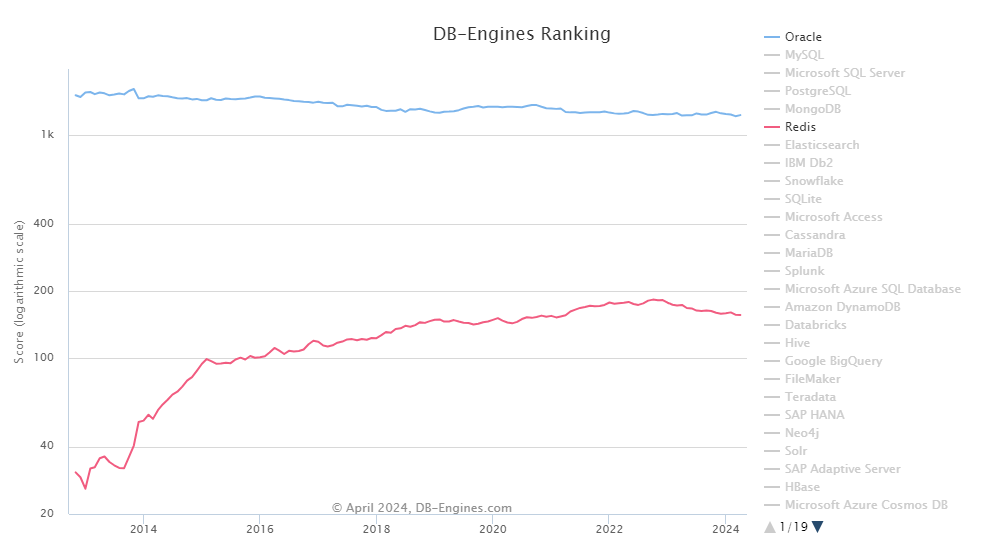
\includegraphics[scale=0.65]{Data/db-engine-trend-dbs.PNG}
		\caption{Graf hodnot popularity RDBS Oracle a KDBS Redis
		\cite{dbranking-trend-by-dbs}\label{graf-dbranking-trend-dbs}}
	\end{figure}

	\begin{figure}[h]
		\centering
		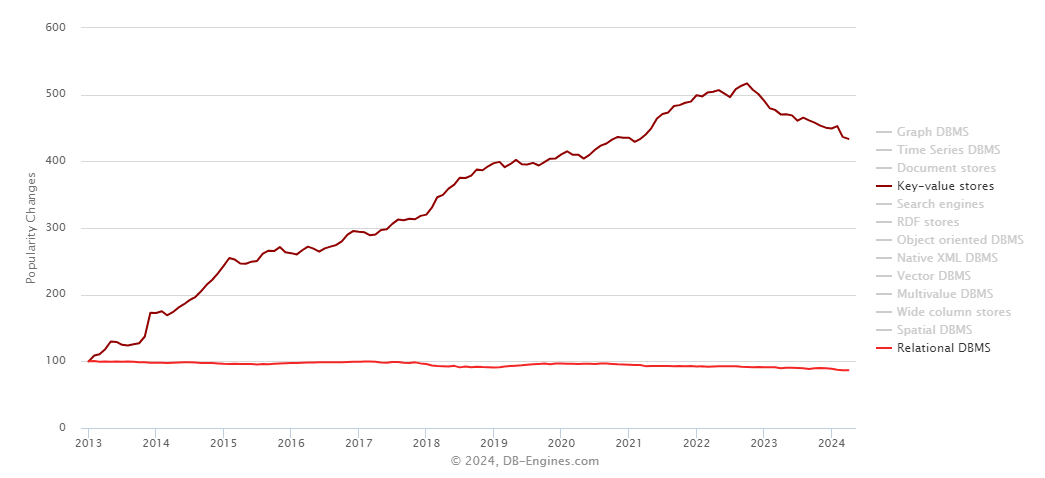
\includegraphics[scale=0.65]{Data/db-engine-trend-model.PNG}
		\caption{Graf změn hodnot popularity RDBS a KDBS \cite{dbranking-trend-by-model}\label{graf-dbranking-trend-model}}
	\end{figure}
	
	\chapter{Key-value databázové systémy\label{chapter:no-sql-ky-sys}}
	
	KDBS~\cite{amaz-key-value-db, ytb-nosql-db, kdbs-oracle, kdbs-redis} jsou typem databázového systému, který se specializuje na ukládání dat ve formě jednoduchých párování klíč-hodnota. Každá hodnota v této databázi je spojena s unikátním klíčem, který slouží k identifikaci daného záznamu (hodnoty). Tyto databáze jsou často preferované pro svou schopnost rychle a efektivně ukládat a získávat data, což je zvláště důležité pro aplikace, které potřebují vysoký výkon a škálovatelnost.
	
	Jedna z hlavních vlastností KDBS spočívá v tom, že ukládají data v jednoduchém formátu klíč-hodnota. Klíč slouží jako identifikátor, který umožňuje rychlé vyhledávání a přístup k datům. Data jsou obvykle indexována podle klíče, což zajišťuje rychlý přístup k nim i při velkém objemu dat.
	
	Důležitým rysem těchto databází je také jejich škálovatelnost. Mohou zpracovávat velké objemy dat a udržovat vysoký výkon i při zvyšujícím se počtu uživatelů nebo objemu dat. Některé systémy KDBS nabízejí distribuované ukládání dat, což umožňuje rozložení dat mezi různé servery a zvýšení odolnosti a výkonu celého systému.
	
	Pro uživatele bývá klíčovým faktorem také jednoduchost použití. KDBS poskytují jednoduché rozhraní pro práci s daty, které zahrnuje základní operace jako vložení, aktualizaci a vyhledávání dat pomocí klíče. Tato jednoduchost usnadňuje integraci DBS do různých aplikací a snižuje nároky na vývojáře.
	
	Vzhledem k těmto vlastnostem jsou KDBS vhodné pro širokou škálu aplikací, včetně webových aplikací, analytických systémů, cache pamětí a dalších. Jsou ideální pro situace, kde je potřeba rychle a efektivně ukládat a získávat data a zároveň udržovat vysoký výkon a škálovatelnost systému.
	
	Jelikož KDBS jsou primárně určeny pro distribuované nasazení, nyní popíšeme tento pojem. Distribuovaný databázový systém~\cite{ddbs} je typ databázového systému, který ukládá data na několik počítačů (neboli uzlů) v rámci sítě. Tento přístup umožňuje přizpůsobitelnější zpracování velkých objemů dat a zlepšuje odolnost systému vůči výpadkům jednotlivých uzlů. Pokud je konkrétní uzel nedostupný kvůli výpadku nebo zvýšené odezvě způsobené přetížením, můžeme jednoduše pokračovat v komunikaci s jiným uzlem, i když je možná vzdálenější. Distribuovaná architektura umožňuje systému růst s rostoucím objemem dat a zároveň snižuje riziko selhání komunikace, což zvyšuje celkovou spolehlivost a dostupnost systému. Dostupnost systému je možné zvýšit například pokrytím rozsáhlejších geografických oblastí vhodným rozmístěním uzlů a přidáním nových uzlů do systému. Tím dosáhneme i kratší odezvy díky možnosti komunikace s uzly blíže uživatelům.
	
	Škálovatelnost~\cite{scalability}\label{scaling-dbs} je schopnost systému přizpůsobit se zvýšené zátěži nebo rostoucímu objemu dat a zachovat požadovanou úroveň výkonu a dostupnosti. Existují různé druhy škálovatelnosti. Horizontální škálovatelnost zahrnuje rozložení zátěže a zvýšení celkové kapacity přidáním dalších uzlů nebo serverů k distribuovanému systému. Vertikální škálovatelnost zlepšuje výkon jednotlivých uzlů nebo serverů zvětšením jejich výpočetní nebo paměťové kapacity. Lineární škálovatelnost je ideální situace, kdy se se zvýšením zdrojů (buď horizontálně nebo vertikálně) zvyšuje výkon systému lineárně.
	
	V současné době existuje celá řada KDBS, od malých open-source projektů po velké komerční cloudové služby. Různé systémy disponují odlišnými vlastnostmi, jako je rychlost zpracování dat, škálovatelnost, uživatelská přívětivost skrze jednoduchou konfiguraci DBS a rozhraní pro práci s daty atd. Dle průzkumu~\cite{predictiveanalyticstoday,g2,db-engineers-ranking} bylo vybráno~9 významných KDBS. Cílem je představit tyto KDBS, popsat jejich klíčové vlastnosti a provést jejich teoretické porovnání (viz tabulka \ref{tab_kvdb_compare}). Z uvedených KDBS se následně provede konečný výběr databází pro testování a porovnání v praxi.
	
	\section{Amazon DynamoDB}
	
	Amazon DynamoDB~\cite{dynamodb} je v současné době druhá nejpopulárnější KDBS~\cite{dynamodb-dbengines-rank2}. Jedná se o cloudový systém bez lokálních serverů (známý též jako serverless cloud systém), který nabízí nízkou odezvu a automatickou škálovatelnost~\cite{dynamodb-autoscaling}. Toho je dosaženo díky správě cloudu ze strany provozovatele a monitoringu běhu databáze. Tento pojem označující databáze v cloudu se používá pro popis architektury, kde se vývojáři především soustředí na vývoj softwaru (aplikace) a provozovatelé cloudu se starají o provoz, škálování a správu infrastruktury bez nutnosti spravovat samostatné servery. Tato KDBS se využitím v oblastech jako je web, technologie IoT, mobilní aplikace a herní průmysl. DynamoDB je plně a automaticky spravovatelná, multi-master databáze zaměřená na vysoké využití horizontální škálovatelnosti. Multi-master databáze~\cite{postgres-multimaster-replication} je typ distribuované databáze umožňující zápis dat na více uzlů současně. Každý uzel má stejná oprávnění k provádění zápisů, které jsou synchronizovány mezi všemi uzly. Tímto způsobem může být zajištěna vyšší dostupnost a odolnost systému proti výpadkům. Pokud jeden uzel selže, ostatní uzly mohou stále zpracovávat zápisy. DynamoDB podporuje různé režimy konzistence dat a umožňuje zápis na více replik v rámci své infrastruktury. Tak jako každá běžná DBS má unikátní primární klíče, které umožňují identifikaci jednotlivých záznamů v tabulkách, tak DynamoDB má i sekundární indexy~\cite{dynamodb-secondary-index} pro zlepšení odezvy dotazů a flexibility, což nebývá běžné pro všechny KDBS. Primární klíč slouží jako vstup do hashovací funkce a výsledná hashovací hodnota určuje fyzickou pozici uloženého záznamu. DynamoDB poskytuje silnou konzistenci při čtení hodnot od poslední aktualizace. Atomické čítače umožňují automatické změny hodnot číselných atributů. Pro expirované záznamy v tabulkách využívá tzv. TTL (Time To Live)~\cite{ttl} k označení doby, po kterou má záznam zůstat platný v databázi. Archivace dat je umožněna díky full backupu. Amazon DynamoDB rovněž nabízí VPC~\cite{vpc} pro soukromou komunikaci za využití vlastní privátní síťové prostředí v rámci AWS cloudu.
	
	Databázový systém disponuje konzolovým API pro správu DBS a práci s daty, ale nabízí také možnost využití jazyka PartiQL~\cite{partiql}, který je vhodný pro kompatibilní SQL dotazy na databázích bez schématu. DynamoDB API je rozděleno do čtyř hlavních částí. Kontrolní plán zahrnuje funkce spojené s vytvářením, úpravami, mazáním a získáním jmen všech tabulek. Dále umožňuje výpis podrobných specifikací dané tabulky, jako jsou primární klíče, indexy a nastavení propustnosti. Následuje datový plán, který poskytuje CRUD operace pro data v dané tabulce. S daty lze pracovat buď jednotlivě po záznamech, nebo pomocí Batch funkcí, které umožňují provést stejnou operaci nad desítkami záznamů najednou a dosáhnout tak vyšší propustnosti, než při volání stejných funkcí pro jednotlivé záznamy opakovaně. Následně je možné provést Scan pro získání všech záznamů dané tabulky nebo indexu, případně Query pro získání hledané části dat. Třetí částí je DynamoDB Streams pro práci s časovými sekvencemi a práci s logy za posledních 24 hodin. Stream API poskytuje funkce pro výpis všech streamů, konkrétní popis daného streamu, získání iterátoru pro daný stream a nakonec získání jednoho záznamu z daného streamu. Poslední částí API jsou ACID transakce, které jsou rozděleny do dvou částí. První část je určena pro batch vkládání, úpravu a mazání záznamů a druhá část slouží k batch získání záznamů.
		
	\section{Oracle NoSQL Database}
	
	Oracle NoSQL Database~\cite{oraclenosqldb} je databázová cloud služba vhodná pro práci s velkými objemy dat a odhadovatelnou nízkou odezvou v řádu jednotek milisekund. Služba je postavena na enginu z Oracle Berkeley DB. Databáze je plně spravovatelná, flexibilní, škáluje horizontálně, dynamicky a dosahuje vysokých výkonů. Mimo Key-value data se jedná i o spolehlivé úložiště pro dokumenty a data s pevně daným schématem. Vzhledem k tomu, že databázový systém je plně spravovaný společností Oracle, tak je pro vývojáře rychlé a snadné začít tuto službu využívat a soustředit se pouze na vývoj aplikací, neboť není potřeba se obtěžovat se správou základní infrastruktury databáze, softwaru, zabezpečení atp. Jedná se o Single Master, Multi Replica grafový systém. Pokud dojde k chybě na masteru, je master automaticky nahrazen jednou z replik. Pro Key-value ukládání s kapacitu jednotek terabytů využívá systém velký počet Storage uzlů, které je možno skupinově konfigurovat. Pro udržení konzistence jsou Storage uzly replikovány. Uzly a hrany v grafu reprezentují entity které vytvářejí vztahy a propojení. Sdílený systém, uniformně alokuje data okolo ostatních částí skupin. Databáze obsahuje i SQL Query s jazykem pro import, export a přenos dat mezi různými Oracle NoSQL databázemi. Mimo jiné je zde podpora i pro Failover, SwitchOver, Bulk Get API, Off Heap Cache a podpora Big Data SQL.
	
	Restové API pro Oracle NoSQL Database je rozděleno do pěti částí. Správa indexů, která dovoluje vytvářet a mazat indexy pro danou tabulku. Tato část API také umožňuje zobrazit všechny indexy, které jsou pro danou tabulku vytvořeny a společně s detailním popisem každého indexu. Druhá část API se věnuje dotazům, umožňuje tedy syntaktickou kontrolu daného SQL dotazu, před připravení a spuštění dotazu. Třetí část je zaměřena na správu záznamů, obsahuje tedy CRUD funkce pro jednotlivé záznamy. Tato část ale neobsahuje funkci pro úpravu existujícího záznamu a ani neumožňuje správu mnoha záznamů najednou, pro úpravu je tedy nutno provést funkci odstranění záznamu a vložení nového a všechny záznamy je tedy také potřeba spravovat jednotlivě a postupně. Čtvrtá část je zaměřena správě tabulek, obsahuje možnost vytvoření, upravování, a mazání tabulek. Tato část také umožňuje výpis všech tabulek, informace o dané tabulce a využívání dané tabulky. Poslední část API se věnuje správě pracovních požadavků, lze zde zobrazit stav jednotlivých požadavků, mazat požadavky, získat chyby či log daného požadavku a list všech požadavků.
		
	\section{Redis} \label{lab-redis}
	
	Redis~\cite{redis} je in-memory úložiště pro datové struktury, využívané jako KDBS, cache, streaming engine nebo zprostředkovatel zpráv. Toto datové úložiště má skvělé využití pro klíče v podobě hashe a hodnoty jako velký JSON objekt. Pro persistenci dat můžeme ukládání dat na disk provádět po nastavitelných pravidelných intervalech, nebo je možné data logovat vždy při vykonávání operací. Pokud nemáme zájem o trvanlivost dat, je možné ukládání dat úplně vypnout a datové úložiště využít čistě jako cache. Úložiště škáluje horizontálně. Redis podporuje datové struktury jako řetězce, hashe, listy, množiny, bitmapy, hyperloglog a geospatial indexy. Nad datovými typy Redis umožňuje rychlé atomické operace, jako je rozšíření řetězců, přidání prvků na začátek a konec listů, atd. Datové úložiště také poskytuje seřazené množiny pro vytváření indexů dle ID nebo jiného číselného atributu. Redis hashing ukládá data jako klíč a mapu. Keyspace notifikace dovoluje klientům odebírat Publisher-Subscriber kanály. Pro práci s dotazy na souřadnice a geometrii je možné využívat Geo API. Redis umožňuje provádět transakce, volat Lua skripty a nastavovat různé úrovně TTL pro záznamy. Redis podporuje Trivial-to-setup Master-Slave asynchronního replikování, společně s rychlou neblokující se prvotní synchronizací. Struktura pro ukládání dat je single-rooted replikovaný strom. Redis má vlastní API pro práci s daty pro populární programovací jazyky jako C, Python, Java a JavaScript.
	
	S Redis databází lze pracovat například pomocí konzolového rozhraní, toto CLI~\cite{rediscli} poskytuje řadu jednoduše čitelných, ale netradičních příkazů pro práci s daty. Vždy potřebujeme specifikovat klíč, se kterým chceme v databázi pracovat. Pomocí příkazu SET a DEL vkládáme do DBS nebo mažeme jednotlivé hodnoty pro zvolený klíč. Příkazem GET získáme hodnoty pro daný klíč, případně můžeme zjistit, zda již existuje záznam pro daný klíč příkazem EXISTS. Pokud vyžadujeme práci s poli, tak můžeme pro daný klíč zleva i zprava vkládat hodnoty zřetězené v poli díky příkazům LPUSH a RPUSH. Obdobně odebíráme hodnoty z pole pomocí LPOP a RPOP, příkazem LRANGE vypíšeme hodnoty z pole a příkazem LLEN zjistíme počet jeho záznamů. Místo jednoduchých polí je možno pracovat i s množinami pomocí příkazů SADD, SREM, SISMEMBER a obdobně. Množiny mohou být i seřazené a pro ně se využívají příkazy jako ZADD. Pro práci se záznamy strukturovanými jako kolekce párů atribut-hodnota se využívá datový typ Hash, umožňuje nám pro daný klíč uložit záznam obsahující názvy atributů a jednotlivé hodnoty pro ně. Opět se zde využívají příkazy jako HSET a HGETALL pro nastavení a získání daného záznamu, případně HGET pro získání hodnoty daného atributu pro záznam na zadaném klíči. API obsahuje také příkazy pro ostatní datové typy, jako jsou bitmapy, geografické prostory, HyperLogLog a další.
	
	\section{Aerospike} \label{lab-aerospike}
	
	Aerospike~\cite{aerospike} je KDBS využívající Hybrid Memory architekturu~\cite{hybmem-arch}, která umožňuje odezvu v jednotkách milisekund a vysokou propustnost v řádech stovek tisíc až milionů operací za sekundu. Hybrid Memory architektura od Aerospike je implementována tak, že index je čistě In-Memory, tím pádem není index perzistentní (vhodné například pro uživatelské cache sessions), a data jsou uložena čistě perzistentně na SSD disku a čtou se přímo z něj. Díky tomu, že je Aerospike jako KDBS naprosto schena-less, je možné definovat Sets a Bins za běhu pro maximální flexibilitu aplikací. Databáze škáluje lineárně a poskytuje silnou konzistenci, nízkou cenu a korektnost. Umožňuje real-time analýzu pro rychlé rozhodování a dynamickou optimalizaci pro vhodné využívání zdrojů dat, proto je databáze vhodná pro velké a stále aktualizované DBS. Poskytuje server-side clustering a bezpečnost na transportní vrstvě. Databáze také umožňuje customer deployment s nulovým downtime. V praxi se Aerospike díky svým vlastnostem využívá například pro banking, telekomunikace, adtech a gaming. Aerospike poskytuje vlastní silný dotazovací jazyk AQL~\cite{aql}, který má prakticky shodnou syntaxi jako SQL (i když se o SQL nejedná). Vlastní vytvořitelné agregační funkce pomocí Lua jazyka jsou flexibilní pro agregační algoritmy.
	
	Dotazovací jazyk AQL se snaží zachovat standardní SQL syntaxi, obvyklé příkazy SELECT, INSERT, DELETE jsou tedy zachovány. Je možné vytvářet vlastní indexy nad tabulkami pomocí CREATE INDEX a provádět agregace pomocí AGGREGATE. Pro dotazy nad konkrétním záznamem specifikovaným pomocí hexadecimálního řetězce či Base64 lze v podmínce dotazu použít porovnání hodnoty s DIGEST nebo EDIGEST. Dotazování můžeme provádět i standardně nad primárním klíčem a ostatními atributy. Při vkládání záznamů lze specifikovat speciální datové typy atributů, jako je LIST, MAP, GEOJSON a další.
	
	\section{Oracle Berkeley DB}
	
	Oracle Berkeley DB~\cite{berkeleydb} je rodina vestavěných Key-value databázových knihoven. Jedná se o čistě In-memory databázi, díky čemuž dosahuje vysokého výkonu a odezvy v jednotkách mikrosekund. Databáze škáluje horizontálně. Data jsou replikována pro vysokou dostupnost z více zdrojů a dobrou toleranci chybovosti. Oracle Berkeley DB využívá vhodné datové struktury pro práci s daty, jako jsou B-strom, hash table indexy nebo fronta. Databáze využívá obnovitelné ACID transakce a poskytuje několik různých úrovní izolace (včetně MVCC~\cite{mvcc}). Data jsou dělena do oddílů dle key ranges. Umožňuje komprimaci dat. Databáze je Single-master, Multi-replica, tedy je vysoce dostupná a umožňuje dobrou konfigurovatelnost. Repliky umožňují čtecí škálovatelnost, rychlý fail-over, hot-standby a další distribuované konfigurace, dodávající podnikové prostředky v malém, vestavěném balíčku. Pro přístup k datům a nastavení databáze se využívá jednoduché volání funkcí API. Mnoho moderních programovacích jazyků, jako například C++, C\#, Java, Python atd., podporuje tyto knihovny. Data mohou být ukládána v nativním formátu aplikace, XML, SQL nebo jako Java objekty. Oracle Berkeley DB je vhodný nástroj pro vše od lokálního úložiště po world-wide distribuovanou databáze (od kilobytů po petabyty).
	
	Interakce s Berkeley DB SQL API je prakticky identická jako s SQLite~\cite{sqlite}. Pro práci s databází vytvořenou rozhraním BDB SQL~\cite{bdbsql} používáte stejná rozhraní API, stejné Shell prostředí, stejné příkazy SQL a stejné PRAGMA, jako se využívá u SQLite. BDB SQL rozšiřuje standardní SQLite PRAGMA o možnosti nastavení velikosti alokované paměti sdílených zdrojů, nastavení počtu bucketů v hashovací tabulce objektů zámků, zvolení soukromého prostředí místo sdíleného, přesměrování logování chyb do vlastního souboru, nastavení příznaku, který způsobí, že sdílené prostředky databáze budou vytvořeny ve sdílené paměti systému a další. Dalším drobným rozdílem je, že BDB SQL rozhraní nepodporuje klíčové slovo IMMEDIATE.
	
	\section{Riak KV} \label{lab-riak}
	
	Riak KV~\cite{riak} je distribuovaná KDBS s pokročilou lokální a multi-cluster replikací, která garantuje čtení a zápis i v případě selhání hardwaru nebo síťových oddílů. Riak využívá bezkonfliktní replikované datové typy (CRDT~\cite{crdt}), které umožňují nezávisle a souběžně aktualizovat jakoukoliv repliku v distribuované databázi se zajištěním sjednocení hodnot pomocí algoritmu, který je součástí samotného datového typu (flagy, registry, čítače, množiny a mapy). Poskytuje konfiguraci aktivního clusteru a dosahuje nízké latence v řádech jednotek milisekund díky dodávání dat z nejbližšího datacentra. Databáze rozděluje data z clusterů pro své dostupné zóny, má multi-cluster repliky a využívá redundance dat v geografickém regionu. Riak tedy automaticky distribuuje data skrz cluster pro robustnost a vysoký výkon. KDBS poskytuje flexibilní datový model bez předem definovaného schématu. Databáze má vylepšené logování chyb a reporty. Data jsou automaticky komprimována pomocí Snappy kompresní knihovny~\cite{snappy}. Databáze využívá master-less architekturu, je vysoce dostupná a má design horizontální škálovatelnosti. Škálovatelnost je téměř lineární při využití snadného přidání hardwarové kapacity bez nutnosti mnoha operací. Riak KV dovoluje zpracování dat pro analýzu a vyvození závěrů pro zlepšení chodu DBS. Riak KV je navržen pro nulové restrikce na hodnoty, takže session data mohou být enkódována mnoha způsoby a nevyžadují změnu schématu. Během nejvyšší zátěže nezhoršuje databáze zápis a horizontální škálovatelnost, uživatelé jsou stále obsluhováni bez problémů. Databáze je vhodná pro ukládání velkého množství nestrukturovaných dat, také pro big-data aplikace, ukládání dat z připojených zařízení a replikaci dat do okolí. Díky nízké latenci je DBS vhodná i pro chat/messaging aplikace. Riak KV exceluje v soukromém, veřejném či hybridním cloud nasazení.
	
	Riak KV API obsahuje všechny potřebné CRUD operace pro správu objektů. Při vytváření nových objektů je potřeba nastavit typ a název bucketu, který skladuje klíče a data do něj vložená. Bucket má také vlastní indexy pro vyhledávání dat uvnitř něj. Dva různé buckety mohou uchovávat stejnou hodnotu klíče, ale jeden bucket obsahuje pouze unikátní klíče. Klíč pro data lze specifikovat explicitně vlastní při vytváření objektu pomocí parametru nebo při jeho absenci je datům přiřazen náhodný klíč. Při vkládání dat do DBS můžeme jednoduše nastavit parametr TTL daného objektu a také počet jeho replik. Při čtení dat můžeme před získáním výsledku zadat minimální počet replik, které se musí shodnout na stejných datech pro zvolený klíč. Pro efektivnější dotazy lze vytvořit vlastní indexy pro výchozí nebo námi zvolená datová schémata. Lze se dotazovat na data pro zvolený klíč nebo provádět fulltextové vyhledávání. Databáze poskytuje i funkce pro tvorbu sekundárních indexů a následné dotazy nad nimi. Riak API také umožňuje hlubší nastavení autorizace a bezpečnosti, práci s replikami a řešení konfliktů.
	
	\section{Voldemort}
	
	Project Voldemort~\cite{voldemort} je distribuovaná KDBS založena na Amazon DynamoDB. Škáluje horizontálně pro čtení i zápis. Umožňuje zapojení storage-enginu (MySQL, Read-Only). Databáze automaticky replikuje data napříč servery pro dostupnost a bezpečnost jednotlivých oddílů při vysoké propustnosti, nicméně každý server obsahuje pouze část z celkových dat. Databáze je decentralizovaná z pohledu uzlů, každý uzel je samostatný a nezávislý, nenachází se zde žádný centrální řídící uzel nebo uzel řídící řešení chyb. Voldemort má výkonost desítek tisíc operací za sekundu na jeden uzel (1 op. za 50 mikrosekund), samozřejmě závisí na hardwaru, síti, systému disku atp. Konzistence dat je nastavitelná (přísné kvórum nebo případná konzistence). Selhání serverů jsou ošetřována transparentně, pro lepší viditelnost, interní monitorování a validaci dat lze využívat JMX~\cite{jmx}. Data jsou verzována pro maximální integritu i během poruch. In-Memory caching pro eliminaci oddělených částí cache, jednoduché a rychlé in-memory testování (např. pro unit testy). Databáze umožňuje jednoduchou distribuci dat skrz stroje, data mohou být rozdělována například dle primárních klíčů. Databáze má hashovatelné schéma, vyhledávání dle primárního klíče a možnost modifikace jednotlivých hodnot. Voldemort poskytuje široké možnosti pro klíče i hodnoty díky serializaci včetně listů a tuplů s pojmenovanými poli. Pro serializaci (Java Serialization, Thrift, Avro) se využívá JSON datový model v kompaktním bytovém formátu, probíhá zde typová kontrola dat dle očekávaného schématu. Pomocí API je možné rozhodovat o replikování a místech ukládání dat, nastavení různé strategie pro specifické aplikace a možnost distribuce dat skrz data centra která jsou mezi sebou geologicky velice vzdálená. Databáze neposkytuje triggery, cizí klíče ani komplexní filtry pro dotazy.
	
	Práce s Voldemort databází z pohledu klienta je přímočará, API se skládá pouze z pár základních funkcí pro správu dat. Tyto funkce jsou Put, Get a Del pro nastavení, získání a odstranění hodnot pro explicitně specifikovaný klíč. Funkce GetAll umožňuje obdržet více hodnot pro více specifikovaných klíčů pomocí volání pouze jedné funkce, GetAll dosahuje vyšší propustnosti než zřetězené volání samostatné funkce Get. Pro připojení k Voldemort databázi a nastavení výchozího uzlu úložiště se využívá funkce Bootstrap, bez nastavení výchozího uzlu je potřeba specifikovat uzel explicitně před každým voláním funkce Get a dalších. Pro funkci Bootstrap je také možné nastavovat serializer pro klíče i hodnoty, čas spojení klienta se serverem a interval automatické změny uzlu v rámci clusteru na ten nejvhodnější. Pro ukončení komunikace se využívá jednoduše funkce Close.
	
	\section{InfinityDB}
	
	InfinityDB~\cite{infinitydb} je NoSQL hierarchicky tříděná KDBS implementovaná v jazyce Java. Databáze má možnost využít čistě In-Memory ukládání dat, která je vhodné pro cache, nebo naopak se mohou data ukládat i perzistentně na disk do souboru, přičemž je možné měnit nastavení bez zasahování do kódu. Přístup k datům v cache je plně vícevláknový, využívá se většina jader, a data, která nejsou často využívaná, jsou stránkována na disk. Databáze dosahuje výkonu v jednotkách milionů operací za sekundu pro více vláknové operace v cache. Veškerá data a informace o databázi jsou uložena na disku v jednom souboru, což zajišťuje jejich aktuálnost a zároveň maximalizuje bezpečnost a korektnost. Databáze je designována právě pro použití jednoho kompletního souboru s okamžitým zotavením a nevyžaduje proto administraci. Databáze neobsahuje dodatečné konfigurační nebo dočasné soubory, upgrade skripty ani logy. Zotavení je bez logů o transakcích okamžité ihned po restartu. V databázi není potřeba dělat čištění junk souborů po operacích, když zde nejsou žádné zanechány. InfinityDB podporuje ACID pro vlákna a ACD pro bulk operace. Databáze poskytuje prostor pro ukládání strukturovaných, polostrukturovaných a nestrukturovaných dat. Tento jednoduchý model umožňuje ukládání vnořených Multi-values a je možné reprezentovat různé datové struktury, jako jsou stromy, grafy, key/value mapy, dokumenty, velká řídká pole a tabulky. Schema je možné měnit za běhu pro zpětnou i následující kompatibilitu. Data dotazů lze dynamicky sledovat pomocí set logic views, delta views a ranges. Databáze se využívá pro servery, pracovní stanice a příruční zařízení.
	
	InfinityDB poskytuje základní jednoduché API o deseti hlavních voláních. Funkcionalitu pro vkládání, úpravu a mazání hodnot zajišťují funkce Insert, Update a Delete. Funkce Delete je rozšířena o funkci Delete-suffixes, která umožňuje odstranit více hodnot v jednom volání. Pro získávání hodnot se využívá kurzoru, jehož pohyb v obou směrech zajišťují funkce First, Next, Last a Previous. Nakonec jsou k dispozici také potřebné funkce Commit a Rollback pro možnost využívání transakcí.
	
	\section{Memcached}
	
	Memcached~\cite{memcached} je open-source, distribuované, in-memory key-value úložiště, navržené pro rychlý a efektivní caching. Primárním účelem Memcached je uchovávání často používaných dat v paměti, aby se snížila latence a zvýšila rychlost přístupu k nim. Jeho jednoduchý a efektivní přístup k ukládání a získávání dat ho činí populární volbou pro webové servery, kde je potřeba rychle cachovat často používané informace jako například HTML stránky, databázové dotazy nebo výpočty. Memcached funguje jako distribuovaná cache, díky čemuž může být nasazen na více serverech, a data jsou mezi nimi rovnoměrně distribuována. Tento přístup umožňuje horizontální škálování, takže kapacitu a výkon Memcached lze jednoduše rozšiřovat přidáním dalších serverů.
	
	Jednou z klíčových vlastností této KDBS je jeho jednoduché API, které podporuje základní operace s key-value páry, jako je ukládání, získávání a mazání dat. Tato funkcionalita je dostupná pomocí funkcí SET, GET, ADD, REPLACE a DELETE. Díky tomu je integrace Memcached do existujících aplikací relativně snadná a není vyžadována žádná složitá konfigurace. Memcached také poskytuje možnost nastavení expirace dat, což umožňuje automatické odstranění zastaralých dat z cache a uvolnění paměťových prostředků. Tato funkce je užitečná zejména pro udržování čerstvých a aktuálních dat v cache. Další významnou vlastností Memcachedu je jeho podpora distribuovaných transakcí, která umožňuje atomické operace nad více key-value páry. Pro práci s touto KDBS jsou k dispozici knihovny pro různé programovací jazyky, což usnadňuje jeho integraci do široké škály aplikací a systémů. Díky své jednoduchosti, efektivitě a škálovatelnosti je Memcached oblíbenou volbou pro mnoho webových aplikací a služeb.

	\begin{sidewaystable}
		\centering
		\caption{Porovnání Key-value databází\label{tab_kvdb_compare}}
		\scalebox{0.8}
		{
			\begin{tabular}{ l|c c c c c c c c } 
				\toprule
				Databáze & Amazon & Oracle & Redis & Aerospike & Oracle & Riak & Voldemort & InfinityDB \\
				& DynamoDB & NoSQL DB & & & Berkeley DB & KV & & \\
				\midrule
				Čistě cloud & ano & ne & ne & ne & ne & ne & ne & ne \\
				Schéma dat & ne & ano i ne & ne & ne & ne & ne & ne & ano \\
				Licence & komerční & open source & open source & open source & open source & open source & open source & komerční \\
				Server OS & hostovaná & Linux, Solaris & Linux, Windows, & Linux & Linux, Windows, & Linux, OS X & Linux, Windows &  Linux, Windows, \\
				& & & OS X, BSD & & OS X, Android ad. & & & OS X, Solaris\\
				Napsáno v & - & Java & C & C & C, C++, Java & Erlang & Java & Java\\
				Sekundární & ano & ano & ano & ano & ano & omezené & ne & ne \\
				indexy & & & & & & & & \\
				Koncept & ACID & ACID & atomické, & atomické & ACID & ne & ne & ACID \\
				transakcí & & v rámci uzlu & izolované & & & & & \\
				Triggery & ano & ne & pub/sub & ne & ano & ano & ne & ne \\
				Dělící & sdílení & sdílení & sdílení & sdílení & ne & sdílení & ne & ne \\ 
				metody \\
				Replikační & ano & source-replica & source-replica, & volitelná & source-replica & volitelný & ne & ne \\
				metody & & multi-region & multi-source & faktor repl. & & faktor repl. \\
				Administrace & vysoká & nízká & vysoká & vysoká & vysoká & vysoká & vysoká & ne\\
				Škálovatelnost & horizontální & horizontální & horizontální & lineární & horizontální & lineární & horizontální & horizontální\\
				Odezva & mikrosekundy & milisekundy & milisekundy & milisekundy & mikrosekundy & milisekundy & milisekundy & milisekundy \\
				Dotazovací & PartiQL & Omezený SQL & Redis & AQL & SQL & Riak & Voldemort & InfinityDB \\
				jazyk & & & query & & & query & query & query \\
				\bottomrule
			\end{tabular}
		}
	\end{sidewaystable}
	
	\section {Nezmíněné významné NoSQL databáze}
	
		Do práce nebyly záměrně zahrnuty databázové systémy MongoDB a Couchbase~\cite{mongodb,couchbase}. I když se jedná o známé a hojně využívané NoSQL databáze, byly obě záměrně vynechány z práce, protože mají Key-value model až jako sekundární datový model. Primárně jsou určeny pro ukládání dokumentově orientovaných informací~\cite{documentdb}. Další často využívanou a nezmíněnou NoSQL databází je Cassandra~\cite{cassandra}, která udává jako datový model wide-column store~\cite{widecolumnstore}. Z tohoto důvodu byla i tato DBS vyřazena z testování.
	
	\chapter{Prostředí pro testování databázových systémů\label{chapter:3-test_environment}}
	
	Různé databázové systémy mohou přistupovat k řešení jednotlivých problémů odlišně. Pokud chceme rozhodnout, který z těchto systémů je nejvhodnější pro určité úkoly, musíme provést řadu testů a porovnání. Je prakticky nemožné nalézt ideální databázový systém, který by exceloval ve všech aspektech pro všechna data a případy využití. Testování nám však umožní odhalit, který systém vyniká a naopak zaostává pro konkrétní operace nad určitými daty. Proto je důležité najít ideální prostředí pro možnost měření a porovnání vlastností vybraných KDBS v kapitole~\ref{chapter:no-sql-ky-sys}.
	
	Existuje celá řada nástrojů pro měření výkonu databázových systémů. Mezi dva dosti známé a dostupné nástroje se řadí například TPC~\cite{tpc} a YCSB~\cite{ycsb}. TPC benchmarky od Transaction Processing Performance Council se dělí do mnoha kategorií. Například TPC-H je považován spíše za benchmark pro systémy pro podporu rozhodování~\cite{dss}, zatímco TPCx-BB je benchmark pro Big Data. Obecně se TPC benchmarky využívají spíše pro typické relační databázové systémy. Na druhou stranu Yahoo! Cloud Serving Benchmark (dále jen YCSB) od společnosti Yahoo! je open-source specifikace a sada programů pro vyhodnocování možností vyhledávání a údržby počítačových programů. Často se ale právě YCSB používá k porovnání relativního výkonu NoSQL databázových systémů, což je pro tuto práci zaměřenou na KDBS ideální. Proto byla tato technologie zvolena pro měření výkonu jednotlivých databázových systémů~\cite{benchmark-pdf-1, benchmark-pdf-2}.
	
	\section{YCSB} \label{lab-ycsb}
	
	YCSB~\cite{ycsb,ycsb-benchmarking} architektura je založena na pluginech a poskytuje snadnou rozšiřitelnost pomocí skriptů. Pro značnou část významných databázových systémů existuje podpora v podobě bindingů. Samotný benchmark se skládá ze dvou fází. První z nich je Loading fáze zaměřená na vložení dat do DBS a následně druhá je Running fáze, ve které se spouští daný test (viz schéma \ref{ycsb-blok-schema}).
	
	Při spouštění každého testu je možné nastavit určité parametry pro lepší konkretizaci měřeného scénáře~\cite{ytb-ycsb}. První a druhý parametr slouží pro specifikaci loading nebo running fáze a výběr testovaného databázového systému. Následně se vybírá testovaný scénář (Workload), počet záznamů v databázi, počet atributů daného záznamu, bytovou velikost každého atributu v záznamu, počet vláken, umístění serveru databáze a nakonec distribuci dotazů (uniformní, exponenciální, sekvenční, nejnovější, hotspot, definované).
	
	YCSB poskytuje 5 různých scénářů označených A až F pro testování propustnosti, latence a škálovatelnosti jednotlivých databázových systémů. Tyto pracovní scénáře, neboli Workloads~\cite{benchmark-pdf-1, workloads}, napodobují různé chování požadavků webových aplikací, jako jsou scénáře zaměřené výhradně na čtení, zápis nebo kombinace obojího. Konkrétní počet zvolených operací dle procentuální definice je vypočítán na základě parametru určujícího celkový počet operací daného scénáře. Při sekvenčním skenování ve Workloadu E je maximální počet skenovaných záznamů v jedné operaci definován jako 5\% z celkového počtu záznamů. Takže při počtu záznamů 1000 bude každá operace skenování číst právě 1 až 50 záznamů.
	
	\begin{itemize} \label{lab-workloads}
		\item Workload A (Update heavy)
		\begin{itemize}
			\item 50\% operací zaměřených na čtení a 50\% operací zaměřených na úpravu
		\end{itemize}
		\item Workload B (Read mostly)
		\begin{itemize}
			\item 95\% operací zaměřených na čtení a 5\% operací zaměřených na úpravu
		\end{itemize}
		\item Workload C (Read only)
		\begin{itemize}
			\item 100\% operací zaměřených na čtení
		\end{itemize}
		\item Workload D (Read latest)
		\begin{itemize}
			\item 95\% operací zaměřených na čtení, 5\% operací zaměřených na vkládání a poslední vložené záznamy jsou čteny přednostně
		\end{itemize}
		\item Workload E (Short ranges)
		\begin{itemize}
			\item 95\% operací zaměřených na sekvenční skenování nízkého počtu záznamů a 5\% operací zaměřených na vkládání
		\end{itemize}
		\item Workload F (Read-modify-write)
		\begin{itemize}
			\item každá operace se skládá z čtení daného záznamu, úpravy záznamu a následného vložení změněného záznamu zpět
		\end{itemize}
	\end{itemize}

	\begin{figure}
		\centering
		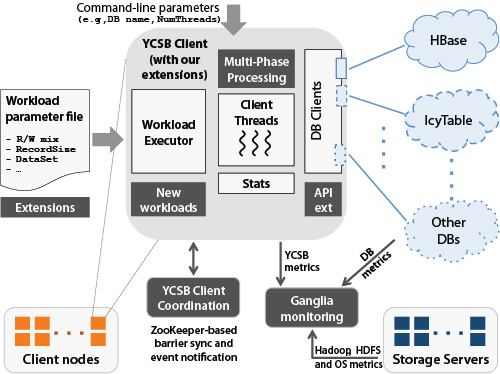
\includegraphics[scale=0.7]{Data/ycsb-1.jpg}
		\caption{YCSB rámec testování funkčnosti \cite{ycsb-parallel-data-lab}\label{ycsb-blok-schema}}
	\end{figure}

	\section{TPC}
	
	Transaction Processing Performance Council~\cite{tpc}, dále jen TPC, je společnost spravující software pro vytváření kvalitních benchmarků výkonnosti systémů pro online zpracování transakcí (OLTP)~\cite{oltp} a možnosti jejich následného monitoringu a porovnávání. TPC benchmarky poskytují spolehlivé testy pro velké firmy s přiměřenou zátěží, výsledkem benchmarků je počet transakcí za minutu (tpm).
	
	TPC benchmarky jsou rozděleny do více modelů pro různě specifikované testy. Prvním z modelů pro OLTP byl TPC Benchmark A (TPC-A), který následně nahradil benchmark TPC-B a aktuálně se v tomto odvětví využívá poslední generace OLTP benchmarků TPC-C a TPC-E. Například modely TPC-DS/DI a TPC-H jsou uzpůsobeny pro benchmark pro systémy pro podporu rozhodování~\cite{dss}. TPC benchmarky jsou přizpůsobeny i pro virtualizaci, IoT~\cite{iot} a další (viz tabulka TPC benchmarků \ref{tab_tpc_modely}).
	
	Model TPC-C~\cite{tpc-c} simuluje velkoobchodní provoz s více sklady, známý jednoduše jako "společnost". V minimálním testu má společnost deset skladů, každý s deseti uživatelskými terminály. Každý sklad obsluhuje deset definovaných prodejních okrsků, každý s 3000 zákazníky, kteří objednávají podle katalogu výrobků o 100 000 položkách. Nejčastějšími transakcemi jsou objednávky zákazníků, přičemž každá objednávka obsahuje v průměru 10 položek, a platby zákazníků. Méně časté požadavky se dotazují na stav objednávek a skladových zásob, expedují objednávky a doplňují zásoby, které se sníží. Pro testování výkonnosti daného systému se počet skladů zvyšuje tak, aby splňoval požadované minimum potřebné k měření cílové úrovně výkonnosti.
	
	Výsledky srovnávacího testu se měří v transakcích za minutu, známých jako tpmC. První výsledek tpmC byl zveřejněn v září 1992 pro IBM AS/400 a přinesl výsledek 54 tpmC. V roce 2000 byl průměrný výsledek pro špičkové stroje 2,4 milionu tpmC a společnosti ve snaze získat rekord stavěly systémy velmi velkých rozměrů. Současný rekord byl stanoven v roce 2020 pomocí cloud computingu, který poskytl 707,3 milionu tpmC~\cite{tpc-c-top-result}. Nedávné výsledky pro menší lokální systémy se zaměřily na snížení nákladů na tpmC.
	
	\begin{table}
		\centering
		\begin{tabular}{ l | l }
			\toprule
			TPC benchmark & využití\\
			\midrule
			TPC-C, TPC-E & zpracovávání transakcí \\
			TPC-H, TPC-DS, TPC-DI & podpora rozhodování \\
			TPCx-V, TPCx-HCI & virtualizace \\
			TPCx-HS, TPCx-BB & velká data \\
			TPCx-IoT & IoT \\
			TPCx-AI & umělá inteligence \\
			TPC-Energy, TPC-Pricing & běžné specifikace \\
			TPC-A, TPC-B, TPC-APP, TPC-D & zastaralé benchmarky \\
			TPC-R, TPC-W, TPC-VMS & \\
			\bottomrule
		\end{tabular}
		\caption{TPC benchmarky\label{tab_tpc_modely}}
	\end{table}
	
	\section{Relevance TPC a YCSB pro měření KDBS}
	
	Pokud jde o relevanci TPC pro KDBS, je potřeba brát v úvahu, že KDBS se liší od tradičních relačních databází. Zatímco TPC benchmarky se zaměřují na transakční zpracování a operace typické pro RDBS, KDBS se často používají pro rychlý přístup k datům pomocí jednoduchého klíč-hodnota rozhraní a jsou často součástí aplikací s vysokým objemem operací typu čtení a zápisu.
	
	Z tohoto důvodu by benchmarky navržené specificky pro KDBS byly relevantnější pro měření jejich výkonnosti a charakteristik. Nicméně některé aspekty TPC benchmarků, jako je schopnost zpracovávat vysoký objem transakcí nebo zátěžové testování, mohou poskytnout užitečné informace i pro KDBS, i když nejsou primárně určeny pro tuto kategorii databází.
	
	Pokud jde o relevanci YCSB pro KDBS, můžeme říci, že je velmi relevantní. To je způsobeno tím, že YCSB je zaměřen na testování databází pomocí jednoduchého klíč-hodnota rozhraní, což je přesně ten způsob, jakým komunikují KDBS.
	
	YCSB poskytuje sadu připravených scénářů a operací, které simuluji reálné aplikace a zátěžové podmínky. To umožňuje uživatelům testovat výkonnost KDBS v různých situacích a porovnávat je s jinými NoSQL DBS. Celkově lze říci, že YCSB je relevantní nástroj pro testování KDBS a poskytuje užitečné informace o jejich výkonu a škálovatelnosti v scénářích podobných reálnému použití.
	
	\chapter{Vyhodnocení výsledků testů\label{chapter:4-test_results}}
	
	\section{Testovací stroj}
	
	Veškeré testy byly spouštěny na vlastním stroji, domácím počítači. Konkrétní specifikace tohoto stroje se nachází v tabulce  (viz tabulka \ref{tab_my_pc_spec}). 
	
	\begin{table}
	\centering
	\caption{Specifikace stroje na kterém se spouštěly testy\label{tab_my_pc_spec}}
		\begin{tabular}{ l | l | l } 
			\toprule
			komponent & název & podrobnosti \\
			\midrule
			OS & Microsoft Windows 10 PRO & x64 \\
			CPU & Intel Core i5 4590 & 3,3GHz (Boost 3,7GHz), core/thread 4, Haswell\\
			GPU & NVIDIA GeForce GTX 1660 SUPER & 6GB, 1530MHz (Boost 1785MHz) \\
			RAM & Crucial Ballistix Sport & 8GB (2x4GB), 1600MHz, DDR3 \\
			SSD & Samsung 870 EVO & R/W 560/530MB/s, 1TB, TLC, SATA 6Gb/s \\
			Základní deska & GIGABYTE GA-H81M-H - Intel H81 & 1150 socket, DDR3 DIMM \\
			\bottomrule
		\end{tabular}
	\end{table}

	\section{Zprovoznění testů}
	
	Pro rozsáhlé otestování byly vybrány čtyři vhodné KDBS. A to konkrétně Redis (\ref{lab-redis}), Riak KV (\ref{lab-riak}), Aerospike (\ref{lab-aerospike}) a Memcached. Všechny tyto zvolené databáze jsou v aktuálním roce 2024 hodnoceny jako jedny z nejlepších podle žebříčku na webu DB-Engines Ranking~\cite{db-engineers-ranking} právě pro testovaný model Key-value. Tento web přiřazuje databázím bodové hodnocení na základě četnosti nových článků o dané databázi na internetu, obecného zájmu, četnosti diskuzí na fórech, množství pracovních nabídek a poptávek a relevanci na sociálních sítích.
	
	Ve snaze o možnost replikace testů byly všechny databáze instalovány a spouštěny pomocí open-source platformy Docker~\cite{docker}. Bylo tedy nutné najít vhodné a kompatibilní docker images pro každou z testovaných databází. V kontextu této práce Docker pomáhá zrychlit zdlouhavou fázi instalování a nastavení počátečního stavu databází, udržení funkčnosti vybrané verze instalovaného softwaru a odstínění od stavu stroje, na kterém DBS spouštíme.
	
	Veškeré testy byly vytvářeny a spouštěny pomocí frameworku YCSB (\ref{lab-ycsb}). YCSB framework v první části, Load, do databáze vložil data, a následně v druhé části, Run, spustil testy a vrátil hodnoty výsledků. Pomocí přidání volitelných parametrů~\cite{ycsb-properties} bylo možné testy upravit podle vlastních potřeb.
	
	Po spuštění databáze v Dockeru se k ní připojil YCSB framework, který následně prováděl testování nad zvolenou připojenou databází. Pro možnost komunikace bylo zapotřebí zprovoznit YCSB binding pro každou z databází, aby YCSB framework mohl úspěšně komunikovat se zvolenou databází, vložit data, spustit testy a vrátit patřičné výsledky.
	
	\section{Popis parametrů testů}
	
	Veškeré testy pro každou z testovaných databází byly spuštěny třikrát, a finální výsledek byl tedy průměrem ze všech tří testů pro každou databázi v dané testovací kategorii. Každý test byl spouštěn paralelně na čtyřech vláknech.
	
	Do databáze bylo vždy vloženo 100~000 záznamů a následující test prováděl 1~000~000 dotazů nad danou naplněnou databází. Následně byla DBS vyprázdněna a celý proces se opakoval ještě dvakrát.
	
	Testy byly prováděny ve třech YCSB kategoriích (tzv. YCSB Workload~\cite{workloads}). Workload A (Update-heavy: 50\% read, 50\% update), Workload B (Read-mostly: 95\% read, 5\% update) a Workload C (Read-only) (viz YCSB Workloads \ref{lab-workloads}).
	
	Pro každý Workload a jednotlivé databáze byla vytvořena tabulka výsledků jednotlivých testů a výsledný průměr těchto testů. Mezi nejdůležitější výsledky testů patří celková doba trvání testu, propustnost a percentily latence operací, konkrétně 95. a 99. percentil. V tabulce jsou také data o počtu provedených operací, průměrné latenci operací, a také minimální, průměrná a maximální latence operací.
	
	Určité databáze vyžadují i další parametry pro spuštění testování, nejčastěji to jsou host IP adresy nebo porty dané DBS pro možné spojení. Dále je například možné specifikovat cestu k souborům, se kterými pracuje testovací prostředí, nebo stanovit TTL~\cite{ttl} testovaných dat, aby bylo možné vyhnout se expiraci dat při dlouhotrvajících nebo vzájemně opožděných testech.
	
	\section{Spouštění testů}
	
	Pro spuštění testů je nejprve zapotřebí nainstalovat, nastavit a spustit vybranou databázi. Poté se musíme k DBS připojit pomocí testovacího prostředí YCSB pro možnou komunikaci s databází a naplnit ji daty. Nakonec spustíme požadované testy a po dokončení testování nám prostředí YCSB vrátí tabulku výsledků v textové podobě.
	
	Nainstalujeme platformu Docker~\cite{docker-console} pro snadnou práci s instalovanými databázemi. Pokud chceme využívat grafického rozhraní pro prostředí Docker, je možnost také instalace platformy Docker Desktop~\cite{docker-desktop, docker-cli} (případně si samozřejmě můžeme DBS instalovat i jiným pro nás vhodnějším způsobem). Docker Desktop bych doporučil pro práci s databázemi, u kterých se plánuje větší úprava konfiguračních souborů nebo sledování chování DBS za běhu prostřednictvím logování.
	
	Práce s Docker Desktop je velice intuitivní, proto se zaměříme na práci s Docker CLI~\cite{docker-cli}. Po zvolení vhodné databáze si musíme stáhnout Docker Image~\cite{docker-image-container} této DBS~\cite{docker-hub} pomocí příkazu "docker~image~pull~[OPTIONS]~NAME[:TAG|@DIGEST]"~\cite{docker-image-pull}. Druhým krokem je nastavení a spuštění DBS. Vytvoříme tedy pomocí Docker Image náš Docker Container~\cite{docker-image-container} který spustíme příkazem "docker~container~run~[OPTIONS]~IMAGE~[COMMAND]~[ARG...]"~\cite{docker-container-run}. Nesmíme zapomenout nastavit správné čísla portů pro Docker Container, jinak nebude testovací prostředí YCSB schopno komunikovat s Docker Image. 
	
	Testovací prostředí YCSB je možné získat z oficiálního GitHub repozitáře Yahoo! Cloud Serving Benchmark~\cite{ycsb}. Pokud nechcete manuálně překládat zdrojové kódy projektu pro možnost nasazení vlastních změn, je vhodné stáhnout funkční verzi, která je k dispozici na odkazu uvedeném v README souboru~\cite{ycsb-download}. Pro úspěšné sestavení projektu ze zdrojových kódů je zapotřebí mít nainstalovaný Apache Maven~\cite{maven} verze 3. Pokud je na stroji nainstalována verze Maven 2, může docházet k chybám (aktuální verzi Mavenu můžete zkontrolovat pomocí příkazu "mvn~-version"). Dále je zapotřebí mít nainstalované Java JDK verze 8 (1.8)~\cite{java-jdk} a vyšší. Na operačním systému Windows doporučuji zkontrolovat hodnotu systémové proměnné "\%JAVA\_HOME\%", abyste se ujistili, že je nastavena správně. To můžete udělat pomocí příkazu "echo~\%JAVA\_HOME\%". Pokud tato systémová proměnná není nastavena správně, musíte ji manuálně změnit (správně nastavená proměnná by měla obsahovat cestu k nainstalovanému Java JDK s verzí minimálně 1.8, například  "C:$\backslash$Program Files$\backslash$Java$\backslash$jdk1.8.0\_231").
	
	Po úspěšném zprovoznění testovacího prostředí YCSB a nastavení DBS, můžeme přejít na poslední fázi testování. Nejprve musíme DBS naplnit daty a následně spustit testy. Veškeré testy byly spouštěny prostřednictvím skriptů vložených do příkazového prostředí Windows PowerShell~\cite{win-powershell}. Nicméně není problém tyto skripty spouštět i v obyčejném příkazovém řádku. Jen zde může nastat problém s čitelností příliš dlouhých výpisů kvůli omezení pohybu ve výpisech. Všechny příkazy byly spouštěny v adresáři "bin", uvnitř kořenového adresáře projektu "ycsb-0.17.0".
	
	V první části testování spustíme příkaz "ycsb~load" pro připojení k databázi a vložení dat do DBS. Nejprve musíme specifikovat název testované DBS a následně zvolený Workload~\cite{workloads}~(viz popis YCSB Workloads~\ref{lab-workloads}). Pomocí volitelných parametrů~\cite{ycsb-properties} na konci každého příkazu specifikujeme naše požadavky. Například počet záznamů, které chceme do DBS vložit, je určen parametrem "-p~recordcount=NUM", počet vláken parametrem "-p~threadcount=NUM", a nejčastěji IP adresa nebo port DBS příkazy "-p~DBS\_NAME.host=IP\_ADR~-p~DBS\_NAME.port=NUM" pro spojení s DBS. Pomocí zadání vlastnosti "-s" po názvu DBS dosáhneme podrobnějšího výstupu při testování včetně chybových hlášek a logů. Celý příkaz pro vložení dat do DBS pak vypadá takto: "ycsb~load~DBS\_NAME~-s~-P~WORKLOAD~[-p~PARAMETERS]". Po dokončení vkládání dat získáme kromě dat v DBS také textový výstup popisující průběh zápisu dat do DBS, kde je zahrnuta propustnost vkládání a čas latence operací rozdělený do sekcí minimum, průměr, maximum a percentily, konkrétně 95. a 99. percentil.
	
	Druhá část testování se věnuje spuštění operací pro čtení a úpravu vložených dat z předchozího kroku pomocí příkazu "ycsb~run". Opět musíme zadat název testované DBS a Workload~\cite{workloads}, který nám určuje poměr operací pro čtení a úpravy dat. Pomocí volitelných parametrů~\cite{ycsb-properties} určíme počet prováděných operací "-p operationcount=NUM". Kombinace celkového počtu operací a Workloadu nám určí konkrétní počet operací čtení a úprav, které se během testu vykonají. Pokud pracujeme s Workloady D nebo E~(viz popis YCSB Workloads~\ref{lab-workloads}), dochází navíc k zápisu nových hodnot do DBS a počet klíčů v DBS stoupá. Ostatní Workloady provádějí pouze úpravy již existujících hodnot, a počet klíčů v DBS zůstává během testu stále stejný. Stejným způsobem jako v první fázi testování, i nyní můžeme specifikovat IP adresu a port DBS, případně počet vláken, podrobnější výstup testu atd. Celý příkaz pro spuštění testu DBS pak vypadá takto: "ycsb~run~DBS\_NAME~-s~-P~WORKLOAD~[-p~PARAMETERS]". Po dokončení testu získáme opět textový výstup v podobě tabulky popisující průběh testu, kde je zahrnuta propustnost operací a čas latence operací rozdělený do sekcí minimum, průměr, maximum a percentily, konkrétně 95. a 99. percentil.
	
	Před reálným testováním můžeme ověřit, zda je všechno správně nastavené, pomocí rychlého dema (viz příkazy~\ref{itemize-demo}). Demo se skládá ze dvou příkazů, naplnění databáze tisíci záznamy a následného otestování, provedení přibližně 500 operací čtení a 500 úprav v databázi BasicDB~\cite{basicdb}. Po spuštění obou příkazů by nám měly testy na konci vrátit status "Return=OK".
	
	\begin{itemize}\label{itemize-demo}
		\item .$\backslash$ycsb load basic -P ..$\backslash$workloads$\backslash$workloada
		\item .$\backslash$ycsb run basic -P ..$\backslash$workloads$\backslash$workloada
	\end{itemize}
	
	Pro názorný příklad si popíšeme a ukážeme příkazy pro testování databáze Redis~\cite{redis} (viz příkazy~\ref{itemiza-docker-ycsb} a obrázky~\ref{ps-docker},~\ref{ps-ycsb-load},~\ref{ps-ycsb-run}). Testovaným scénářem bude Workload A~\cite{workloads} (50\% Read, 50\% Update), který poběží na 4 vláknech. Do databáze se vloží 10~000 záznamů, a provede se 10~000 operací během testování (přibližně 5~000 čtení a 5~000 aktualizací dat). Nejprve si stáhneme Docker Image pro KDBS Redis příkazem "docker pull" a následně spustíme kontejner příkazem "docker run" a nastavíme porty. Nyní máme DBS připravenou a můžeme začít s testováním. Nejprve spustíme příkaz "ycsb load" k vložení dat do databáze. Po dokončení vkládání dat můžeme v příkazovém řádku vidět tabulku popisující informace o vkládání dat do databáze. Následně zahájíme testy spuštěním příkazu "ycsb run", a opět uvidíme ve výstupní tabulce výpis informací o našem testu. Pokud na konci tabulky uvidíme status "Return=OK", vše proběhlo podle očekávání.
	
	\begin{itemize}\label{itemiza-docker-ycsb}
		\item docker pull redis:latest
		\item docker run --name my-redis -p 6379:6379 -d redis:latest
		\item .$\backslash$ycsb load redis -P  ..$\backslash$workloads$\backslash$workloada -p redis.host=127.0.0.1 -p redis.port=6379 \\-p recordcount=10000 -p threadcount=4
		\item .$\backslash$ycsb run redis -P ..$\backslash$workloads$\backslash$workloada -p redis.host=127.0.0.1 -p redis.port=6379 \\-p operationcount=10000 -p threadcount=4
		\item docker stop aba5fabc123example4568aa97
		\item docker rm aba5fabc123example4568aa97
	\end{itemize}
	
	\lstdefinestyle{DOS}
	{
		backgroundcolor=\color[RGB]{1, 36, 86},
		basicstyle=\scriptsize\color{white}\ttfamily
	}
	
	\begin{figure}
	\centering
	\begin{lstlisting}[style=DOS]
	PS E:\ycsb-0.17.0\bin> docker pull redis:latest
	latest: Pulling from library/redis
	Digest: sha256:f14f42fabc123example456c7e824b9
	Status: Image is up to date for redis:latest
	docker.io/library/redis:latest
		
	PS E:\ycsb-0.17.0\bin> docker run --name my-redis -p 6379:6379 -d redis:latest
	aba5fabc123example4568aa97
		
	PS E:\ycsb-0.17.0\bin> docker stop aba5fabc123example4568aa97
	aba5fabc123example4568aa97
		
	PS E:\ycsb-0.17.0\bin> docker rm aba5fabc123example4568aa97
	aba5fabc123example4568aa97
	\end{lstlisting}
	\caption{Docker Redis, příkazy pro stažení, spuštění, zastavení a odstranění DBS
	\label{ps-docker}}
	\end{figure}
	
	\begin{figure}
	\centering
	\begin{lstlisting}[style=DOS]
	PS E:\ycsb-0.17.0\bin> .\ycsb load redis -P ..\workloads\workloada
		-p redis.host=127.0.0.1 -p redis.port=6379 -p recordcount=10000
		-p threadcount=4
	YCSB Client 0.17.0
	Loading workload...
	Starting test.
	[OVERALL], RunTime(ms), 4211
	[OVERALL], Throughput(ops/sec), 2374.7328425552128
	[TOTAL_GCS_PS_Scavenge], Count, 4
	[TOTAL_GC_TIME_PS_Scavenge], Time(ms), 6
	[TOTAL_GC_TIME_%_PS_Scavenge], Time(%), 0.14248397055331277
	[TOTAL_GCS_PS_MarkSweep], Count, 0
	[TOTAL_GC_TIME_PS_MarkSweep], Time(ms), 0
	[TOTAL_GC_TIME_%_PS_MarkSweep], Time(%), 0.0
	[TOTAL_GCs], Count, 4
	[TOTAL_GC_TIME], Time(ms), 6
	[TOTAL_GC_TIME_%], Time(%), 0.14248397055331277
	[CLEANUP], Operations, 4
	[CLEANUP], AverageLatency(us), 333.25
	[CLEANUP], MinLatency(us), 80
	[CLEANUP], MaxLatency(us), 1060
	[CLEANUP], 95thPercentileLatency(us), 1060
	[CLEANUP], 99thPercentileLatency(us), 1060
	[INSERT], Operations, 10000
	[INSERT], AverageLatency(us), 1647.61
	[INSERT], MinLatency(us), 904
	[INSERT], MaxLatency(us), 13895
	[INSERT], 95thPercentileLatency(us), 2481
	[INSERT], 99thPercentileLatency(us), 3389
	[INSERT], Return=OK, 10000
	\end{lstlisting}
	\caption{YCSB Redis, příkaz pro vložení dat (load)
	\label{ps-ycsb-load}}
	\end{figure}

	\begin{figure}
	\centering
	\begin{lstlisting}[style=DOS]
	PS E:\ycsb-0.17.0\bin> .\ycsb run redis -P ..\workloads\workloada
		-p redis.host=127.0.0.1 -p redis.port=6379 -p operationcount=10000
		-p threadcount=4
	YCSB Client 0.17.0
	Loading workload...
	Starting test.
	[OVERALL], RunTime(ms), 2560
	[OVERALL], Throughput(ops/sec), 3906.25
	[TOTAL_GCS_PS_Scavenge], Count, 1
	[TOTAL_GC_TIME_PS_Scavenge], Time(ms), 1
	[TOTAL_GC_TIME_%_PS_Scavenge], Time(%), 0.0390625
	[TOTAL_GCS_PS_MarkSweep], Count, 0
	[TOTAL_GC_TIME_PS_MarkSweep], Time(ms), 0
	[TOTAL_GC_TIME_%_PS_MarkSweep], Time(%), 0.0
	[TOTAL_GCs], Count, 1
	[TOTAL_GC_TIME], Time(ms), 1
	[TOTAL_GC_TIME_%], Time(%), 0.0390625
	[READ], Operations, 5157
	[READ], AverageLatency(us), 998.8885010665116
	[READ], MinLatency(us), 389
	[READ], MaxLatency(us), 17695
	[READ], 95thPercentileLatency(us), 1692
	[READ], 99thPercentileLatency(us), 3479
	[READ], Return=OK, 5157
	[CLEANUP], Operations, 4
	[CLEANUP], AverageLatency(us), 221.75
	[CLEANUP], MinLatency(us), 60
	[CLEANUP], MaxLatency(us), 638
	[CLEANUP], 95thPercentileLatency(us), 638
	[CLEANUP], 99thPercentileLatency(us), 638
	[UPDATE], Operations, 4843
	[UPDATE], AverageLatency(us), 985.7646087136072
	[UPDATE], MinLatency(us), 364
	[UPDATE], MaxLatency(us), 17567
	[UPDATE], 95thPercentileLatency(us), 1744
	[UPDATE], 99thPercentileLatency(us), 3675
	[UPDATE], Return=OK, 4843
	\end{lstlisting}
	\caption{YCSB Redis, příkaz pro spuštění testů (run)
	\label{ps-ycsb-run}}
	\end{figure}

	\section{Vyhodnocení výsledků testů}
	
	Po opětovném spouštění stejných testů a následném zprůměrování naměřených hodnot jsme došli k finálním výsledkům. Hlavní měřené parametry byly propustnost (počet operací za sekundu), celkový čas testu (milisekundy), a minimální, průměrná, maximální latence na operaci (mikrosekundy) a percentil latence (mikrosekundy), konkrétně 95. a 99. percentil.
	
	Jednotlivé testy se dělí do 4 scénářů Workload A, Workload B, Workload C a Insert only (viz~\ref{lab-workloads}). Pro každý scénář se otestovaly všechny 4 vybrané KDBS třikrát, a následně se výsledky dané KDBS pro daný scénář zprůměrovaly. U scénářů Workload A a Workload B se měřila latence čtení a úpravu dat zvlášť, proto se výsledná latence těchto dvou scénářů počítala jako průměr latence pro čtení a úpravu dat. Workload C provádí pouze čtení dat, proto nebylo zapotřebí průměrovat latence mezi sebou a stejně tak tomu je i u scénáře kde se pouze plní KDBS daty (Insert only). U grafů a tabulek latence je minimum označeno zkratkou "min", maximum "max" a průměr "avg".
	
	V grafech porovnávajících propustnosti KDBS jsem zavedl jednotku "kiloops/sec" reprezentující tisíce operací za sekundu. Všechny měřené propustnosti se pohybují v řádech jednotek tisíců operací za sekundu, proto je tato jednotka vhodná a zlepšuje čitelnost grafů. Nejvyšší naměřené hodnoty latence jsem zařadil do jednoho společného grafu napříč všemi testovými scénáři (viz graf~\ref{graph_Workloads A, B, C + Insert only - Max Latency (ms)}) protože při porovnání maximální latence v jednom grafu daného scénáře s minimální a průměrnou latencí (viz graf~\ref{graph_Workload A - Min Avg Latency (ms)}) docházelo k velkému nepoměru vykreslených hodnot který jednou kategorií maximálních hodnot způsoboval zanedbatelné vizuální rozdíly pro hodnoty nejnižší a průměrné z předešlých kategorií. Při použití logaritmické stupnice nebyly grafy stále čitelné, proto jsem maximální latence dal do jednoho společného grafu napříč všemi testovými scénáři. Pokud na sloupcovém grafu dochází k několikanásobnému převýšení jedné maximální hodnoty některého sloupce vůči sloupcům ostatním v rámci dané kategorie či celého grafu využívám vizuální indikátor přetrhnutého sloupce (viz graf~\ref{graph_Workload B - Percentile Latency (ms)}), který znázorňuje že daný sloupec je vyšší oproti ostatním a zároveň nedochází k vykreslení celé výšky sloupce pro možnost zachovat vizuální poměry ostatních několikanásobně nižších hodnot.
	
	V rámci všech testů KDBS Riak KV několikanásobně zaostávala vůči zbylým třem databázím. Při testování docházelo i k pádům samotné KDBS spouštěné v Dockeru, a obecně docházelo k chybám a přetékání paměti způsobené nejspíše špatným nastavením konfiguračních souborů, obecně nastavení této KDBS bylo nejtěžší v porovnání s ostatními. Ve výsledcích testů (viz tabulka~\ref{tab_workload_a}) můžeme vidět, že KDBS Riak KV má hodnotu nejnižší latence stále vyšší než jsou průměrné latence zbylých tří databází a dokonce je i vyšší než 95. percentil latence zbylých KDBS.
	
	\subsection{Testový scénář 1 - Workload A}
	
	Prvním testovaným scénářem byl Workload A~\cite{workloads}, scénář se skládá z 50 \% operací pro čtení a 50 \% pro aktualizaci dat. Tento scénář byl vybrán pro demonstraci chování databází při vysokém počtu operací zaměřených právě na úpravu dat. Do každé KDBS bylo předem vloženo 100~000 záznamů a provádělo se 1~000~000 testovacích operací. Tedy přibližně 500~000 čtení a 500~000 úprav, konkrétní počet poměru operací se vždy liší v řádu nízkých stovek (v součtu je vždy roven milionu).
	
	Z naměřených hodnot (viz tabulka~\ref{tab_workload_a} a grafy~\ref{graph_Workloads A, B, C + Insert only - Throughput (kiloops/sec)},~\ref{graph_Workloads A, B, C + Insert only - Runtime(s)}) můžeme vidět že databáze Aerospike dosáhla nejvyšší propustnosti ze všech měřených KDBS 5081,13 operací za sekundu a její testy trvaly průměrně 196,8 sekund. Databáze Redis se umístila hned jako druhá s propustností 4801,04 operací za sekundu. Propustnost KDBS Redis je průměrně menší o 5,51 \% oproti KDBS Aerospike pro scénář Workload A. Následuje KDBS Memcached s propustností 4108,70 operací za sekundu, která oproti KDBS Aerospike zaostává o 19,13 \% a při srovnání s KDBS Redis je to méně o 14,42 \%. Nakonec KDBS Riak KV dosáhla nejnižší propustnosti 1283,98 operací za sekundu, což je zhoršení o 74,73 \% oproti KDBS Aerospike. Riak KV je pro tento scénář téměř čtyřnásobné pomalejší ve srovnání s nejrychlejší měřenou databází Aerospike.
	
	Při porovnání latence operací na první pohled vidíme že trend rychlostí latence operací kopíruje propustnosti. Pokud se zaměříme na minimální a průměrnou latenci (viz graf~\ref{graph_Workload A - Min Avg Latency (ms)}), tak vidíme že KDBS Aerospike zpracovala operaci nejrychleji za 317 $\mu$s a KDBS Redis za 315,17 $\mu$s. Rozdíl v minimální latenci pro tyto dvě KDBS je zanedbatelný. Databáze Memcached má poté minimální latenci operace 401,5 $\mu$s, tedy přibližně o 27 \% při porovnání s KDBS Aerospike a Redis. Databáze Riak KV má nejnižší latenci 1694 $\mu$s, což je pětinásobně více než nejnižší latence v tomto měření. Minimální latence KDBS Riak KV převyšuje i průměrné latence a 95. percentily tří zbylých databází ve všech testech pro tento scénář. Z toho měření vyplývá že pro tento scénář a konfiguraci má KDBS Riak KV několikanásobně vyšší latenci operací. U průměrné latence vidíme že KDBS Aerospike a Redis dosahují podobných hodnot přibližně 800 $\mu$s. KDBS Memcached dosahuje průměrné latence 967,9 $\mu$s což je opět o 23,31 \% pomalejší ve srovnání s KDBS Aerospike.
	
	Z největších naměřených latencí (viz graf~\ref{graph_Workloads A, B, C + Insert only - Max Latency (ms)}) můžeme vidět že KDBS Aerospike provedla nejpomalejší operaci za 28,53 ms. V nejhorším možném případě pro tento scénář z hlediska latence operací byla KDBS Aerospike rychlejší přibližně o 67,94 \% oproti KDBS Redis u které maximální latence činí 47,92 ms a přibližně o 190 \% při porovnání s KDBS Memecached kde byla maximální latence 82,71 \%. KDBS Riak KV je dosáhla nejvyšší latence 163,02 ms a je skoro dvojnásobně pomalejší při porovnání v rámci tohoto měření s druhou nejpomalejší KDBS Memcached.
	
	Pokud se zaměříme na 95. a 99. percentil latence (viz graf~\ref{graph_Workload A - Percentile Latency (ms)}) tak je zřejmé že KDBS Aerospike dominuje svou nízkou latencí i v této kategorii pro scénář Workload A. KDBS Aerospike má 95. percentil 1121,8 $\mu$s, což je o 11,81 \% méně při srovnání s 95. percentilem KDBS Redis který činí 1273 $\mu$s a o 19,42 \% oproti KDBS Memcached kde 95. percentil latence 1386,33 $\mu$s. Nakonec KDBS Riak KV dosáhla 95. percentilu latence 6757 $\mu$s. Hodnota pro 99. percentil latence KDBS Aerospike byla 1539,33 $\mu$s, což je opět nejnižší 99. percentil latence napříč všemi KDBS v rámci tohoto scénáře. Databáze Memcached má druhý nejnižší 99. percentil latence s hodnotou 1848,33 $\mu$s a těsně za ní následuje KDBS Redis s 99. percentilem latence 1904,5 $\mu$s. KDBS Aerospike má 99. percentil nižší o 16,76 \% při srovnání s KDBS Memcached a o 18,95 \% menší při srovnání s KDBS Redis. KDBS Riak KV má opět nejhorší výsledky, a to latency 11,87 $\mu$s pro 99. percentil.
	
	Z naměřených hodnot testového scénáře Workload A můžeme vidět že KDBS Aerospike zvládá nejlépe velký počet aktualizací ve srovnání s ostatními testovanými KDBS. Databáze Aerospike dosahovala výsledků přibližně o 15 \% lepších při srovnání s ostatními KDBS. Za ní následovaly KDBS Redis a Memcached které měli vzájemně podobné výsledky. Databáze Redis byla v řádu jednotek procent lepší oproti Memcached ve všech měřeních s výjimkou 99. percentilu latence kde byla KDBS Memcached lepší o 3,04 \% (viz graf~\ref{graph_Workload A - Percentile Latency (ms)}). Jediná databáze Riak KV několikanásobně zaostávala vůči všem ostatním testovaným KDBS v rámci všech naměřených hodnot. Pokud bychom se zaměřili zvlášť na operace čtení a aktualizací u KDBS Riak KV (viz tabulka~\ref{tab_workload_a}) tak uvidíme že latence aktualizací je minimálně dvojnásobně horší než latence čtení pro tuto KDBS, oproti tomu ostatní testované KDBS v rámci tohoto scénáře dosahovaly téměř identické latence jak pro čtení tak zápis.
	
	\begin{table}
		\centering
		\begin{tabular}{ l | l l l l }
			\toprule
			KDBS & Redis & Riak KV & Aerospike & Memcached \\
			\midrule
			Čas běhu (ms) & 208419 & 803880,33 & 196849,33 & 243409,33 \\
			Propustnost (op/sec) & 4801,04 & 1283,98 & 5081,13 & 4108,70 \\
			\midrule
			\multicolumn{5}{l}{Čtení} \\
			Počet operací & 500157 & 500382 & 499106 & 500683 \\
			Avg letence ($\mu$s) & 836,77 & 2175,86 & 785,86 & 967,90 \\
			Min letence ($\mu$s) & 325,33 & 861,33 & 319,67 & 395,33 \\
			Max letence ($\mu$s) & 50473,67 & 158271 & 27311 & 83177,67 \\
			Letence 95. percentil ($\mu$s) & 1281,33 & 3695 & 1122,67 & 1385 \\
			Letence 99. percentil ($\mu$s) & 1917,33 & 7399 & 1540,33 & 1846 \\
			\midrule
			\multicolumn{5}{l}{Aktualizace} \\
			Počet operací & 499843 & 499618 & 500894 & 499317 \\
			Avg letence ($\mu$s) & 824,13 & 5941,33 & 782,68 & 967,90 \\
			Min letence ($\mu$s) & 305 & 2526,67 & 314,33 & 407,67 \\
			Max letence ($\mu$s) & 45375 & 167764,33 & 29753,67 & 82249,67 \\
			Letence 95. percentil ($\mu$s) & 1264,67 & 9819 & 1121 & 1387,67 \\
			Letencezva 99. percentil ($\mu$s) & 1891,67 & 16332,33 & 1538,33 & 1850,67 \\
			\midrule
			\multicolumn{5}{l}{Čtení + aktualizace} \\
			Počet operací & 1000000 & 1000000 & 1000000 & 1000000 \\
			Avg letence ($\mu$s) & 830,45 & 4058,59 & 784,27 & 967,90 \\
			Min letence ($\mu$s) & 315,17 & 1694 & 317 & 401,5 \\
			Max letence ($\mu$s) & 47924,3 & 163017,67 & 28532,33 & 82713,67 \\
			Letence 95. percentil ($\mu$s) & 1273 & 6757 & 1121,83 & 1386,33 \\
			Latence 99. percentil ($\mu$s) & 1904,5 & 11865,67 & 1539,33 & 1848,33 \\
			\bottomrule
		\end{tabular}
		\caption{Naměřené výsledky testů pro Workload A\label{tab_workload_a}}
	\end{table}
	
	\subsection{Testový scénář 2 - Workload B}
	
	Druhým testovaným scénářem byl Workload B~\cite{workloads}, tento scénář se snaží více realisticky simulovat reálná chod databázového systému v praxi, kde většinou dochází především ke čtení záznamům a aktualizace jsou oproti tomu poměrově méně frekventované. Tento scénář se skládá z 95~\% operací zaměřených na čtení a 5~\% aktualizací. Oproti prvnímu scénáři kde byl poměr těchto dvou operací vyvážený (50~\% čtení, 50~\% aktualizace) bude tento scénář více přizpůsobený databázím které disponují rychlím čtením a pomalé aktualizace zde nebudou tvořit tak znatelné omezení. Do každé KDBS bylo předem vloženo 100~000 záznamů a provádělo se 1~000~000 testovacích operací. Tedy přibližně 950~000 čtení a 50~000 úprav, konkrétní počet poměru operací se vždy liší v řádu nízkých stovek (v součtu je vždy roven milionu).
	
	Z naměřených hodnot (viz tabulka~\ref{tab_workload_b}) můžeme vidět že i pro druhý scénář se nám opakuje stejný trend propustností KDBS dle propustnosti jako tomu bylo u prvního scénáře. Pokud se podíváme na grafy propustnosti a celkového času běhu testu (viz grafy~\ref{graph_Workloads A, B, C + Insert only - Throughput (kiloops/sec)},~\ref{graph_Workloads A, B, C + Insert only - Runtime(s)}) tak zjistíme že KDBS Aerospike opět dosáhla nejlepší propustnosti napříč všemi testovanými KDBS která se rovná 4945,37 operací za sekundu a průměrným časem běhu celého testu 202,3 sekund. KDBS Aerospike má o 4,62~\% lepší propustnost při porovnání s KDBS Redis, o 27,99~\% oproti KDBS Memcached a o 178,18~\% oproti KDBS Riak KV. Na druhém místě co se týče propustnosti je stejně jako v předešlém scénáři KDBS Redis s propustností 4726,96 operací za sekundu. Dále následuje KDBS Memcached s hodnotou propustnosti 3863,59 operací za sekundu a nakonec stejně jako v předešlém scénáři KDBS Riak KV s propustností 1778,16 operací za sekundu.
	
	Z grafu minimální a průměrné latence operace (viz graf~\ref{graph_Workload B - Min Avg Latency (ms)}) vyplývá že KDBS Aerospike a Redis mají prakticky identické časy latence nejkratší operace a to 327 $\mu$s, liší se pouze v desetinných hodnotách což je zanedbatelný rozdíl. Následuje KDBS Memcached s nejmenší latencí 397,83 $\mu$s zaostávající o 17,71~\%. Poslední je KDBS Riak KV s nejvyšší hodnotou minimálního času latence operace 1795,33~$\mu$s pomalejší o 81,78~\%. Průměrné časy latence operací jsou pro KDBS Aerospike a Redis opět téměř identické s hodnotou 807,98~$\mu$s pro Aerospike a 843,29~$\mu$s pro Redis. Následuje KDBS Memcached s hodnotou 1055,21~$\mu$s která je o 30,60~\% větší než je tomu pro KDBS Aerospike. Nakonec KDBS Riak KV dosáhla nejmenšího latence 3950,21~$\mu$s což je o 388,95~\% víc při porovnání s KDBS Aerospike.
	
	Nejvyšší hodnoty latence (viz graf~\ref{graph_Workloads A, B, C + Insert only - Max Latency (ms)}) ukazují v tomto případě oproti scénáři Workload A velký nárůst pro KDBS Memcached (101,82~ms) a naopak pokles pro KDBS Riak KV (118,79~ms). Databáze Aerospike a Redis se drží na hodnotách velice blízkým předešlému scénáři. To znamená že KDBS Aerospike dosahuje hodnoty maximální latence 21,43~ms což je o 53,41~\% méně při porovnání s KDBS Redis kde je maximální hodnota latence 46~ms.
	
	Při zaměření na porovnání percentilů latencí (viz graf~\ref{graph_Workload B - Percentile Latency (ms)}) vidíme že i 95. a 99. percentil latence následuje trend ostatních výsledků tohoto testovaného scénáře. KDBS Aerospike má 95. percentil latence roven 1192,83~$\mu$s. Tento percentil je nižší o 9,87~\% při srovnání s KDBS Redis která má 95. percentil latence roven 1323,67~$\mu$s. Oproti KDBS Memcached pro kterou je 95. percentil latence roven 1744~$\mu$s je KDBS Aerospike rychlejší o 31,61~\%. Při porovnání s KDBS Riak KV vidíme obrovský skok na 95. percentil latence roven 6067,67~$\mu$s což je přibližně o 409~\% více oproti KDBS Aerospike a o 247,98~\% oproti KDBS Memcached která je v rámci tohoto scénáře druhá nejpomalejší. Při sledování 99. percentilu vidíme opět stejné poměry hodnot, nejnižší hodnota u KDBS Aerospike činí 1767,83~$\mu$s, následuje Redis s 2237,83~$\mu$s a zhoršením o 26,60~\% oproti Aerospike, poté Memcached s 2838~$\mu$s a nakonec opět Riak KV s 99. percentilem latence 10650,33~$\mu$s.
	
	Z tohoto měření vyplývá že KDBS Memcached pro scénář Workload B zaostává oproti databázím Aerospike a Redis. Samotné KDBS Aerospike a Redis mají stejně jako v předešlém scénáři vzájemně podobné výsledky pro všechny měřené kategorie, i přesto Aerospike dosahuje lepších výsledků i když jen v zanedbatelných řádech. Databáze Riak KV dosahuje stále řádově horších hodnot oproti ostatním testovaným KDBS, každopádně si vede lépe než tomu bylo v předešlém scénáři, propustnost se navýšila o 494,19 operací za sekundu což činí zlepšení o 38,43~\%, zbylé 3 KDBS si vedli srovnatelně s předešlým scénářem. Z toho scénáře vyplývá že KDBS Riak KV znatelně zaostává při aktualizacích, proto nyní dochází ke zvýšení propustnosti při sníženém počtu aktualizací. Na druhou stranu KDBS Memcached při sníženém počtu aktualizací zaostává oproti předešlému scénáři o 6,08~\% protože nemá dostatečně rychlé čtení při srovnání s KDBS Aerospike a Redis.
	
	\begin{table}
		\centering
		\begin{tabular}{ l | l l l l }
			\toprule
			KDBS & Redis & Riak KV & Aerospike & Memcached \\
			\midrule
			Čas běhu (ms) & 212026,33 & 562799,67 & 202264 & 263195,67 \\
			Propustnost (op/sec) & 4726,96 & 1778,16 & 4945,38 & 3863,59 \\
			\midrule
			\multicolumn{5}{l}{Čtení} \\
			Počet operací & 949836 & 949728 & 949706 & 950435 \\
			Avg letence ($\mu$s) & 845,22 & 2072,91 & 805,97 & 1046,18 \\
			Min letence ($\mu$s) & 313,67 & 825,33 & 313,33 & 389 \\
			Max letence ($\mu$s) & 50559 & 110356,33 & 25732,33 & 112020,33 \\
			Letence 95. percentil & 1325 & 3232,33 & 1188 & 1735,33 \\
			Letence 99. percentil ($\mu$s) & 2232,33 & 6805,67 & 1756 & 2813 \\
			\midrule
			\multicolumn{5}{l}{Aktualizace} \\
			Počet operací & 50164 & 50272 & 50294 & 49565 \\
			Avg letence ($\mu$s) & 841,3802758 & 5827,51 & 809,98 & 1064,24 \\
			Min letence ($\mu$s) & 342 & 2765,33 & 341,33 & 406,67 \\
			Max letence ($\mu$s) & 41449,67 & 127231 & 17132,33 & 91625,67 \\
			Letence 95. percentil & 1322,33 & 8903 & 1197,67 & 1752,67 \\
			Letence 99. percentil ($\mu$s) & 2243,33 & 14495 & 1779,67 & 2851 \\
			\midrule
			\multicolumn{5}{l}{Čtení + aktualizace} \\
			Počet operací & 1000000 & 1000000 & 1000000 & 1000000 \\
			Avg letence ($\mu$s) & 843,30 & 3950,21 & 807,97 & 1055,21 \\
			Min letence ($\mu$s) & 327,83 & 1795,33 & 327,33 & 397,83 \\
			Max letence ($\mu$s) & 46004,33 & 118793,67 & 21432,33 & 101823 \\
			Letence 95. percentil & 1323,67 & 6067,67 & 1192,83 & 1744 \\
			Letence 99. percentil ($\mu$s) & 2237,83 & 10650,33 & 1767,83 & 2832 \\
			\bottomrule
		\end{tabular}
		\caption{Naměřené výsledky testů pro Workload B\label{tab_workload_b}}
	\end{table}
	
	\subsection{Testový scénář 3 - Workload C}
	
	Třetím testovým scénářem je Workload C~\cite{workloads}. Tento scénář se věnuje čistě čtení záznamů. Výsledky tohoto scénáře nám pomohou porovnat propustnost testovaných KDBS čistě na základě načítání hodnot, pokud má databáze velice rychlé čtení ale pomalé zápisy, aktualizace nebo mazání hodnot tak v tomto scénáři bude excelovat. Do každé KDBS bylo předem vloženo 100~000 záznamů a testovalo se 1~000~000 operací čtení hodnot.
	
	\begin{table}
		\centering
		\begin{tabular}{ l | l l l l }
			\toprule
			KDBS & Redis & Riak KV & Aerospike & Memcached \\
			\midrule
			Čas běhu (ms) & 205492,67 & 562029,33 & 209528 & 221353,33 \\
			Propustnost (op/sec) & 4868,30 & 1783,39 & 4778,13 & 4517,67 \\
			\midrule
			\multicolumn{5}{l}{Čtení} \\
			Počet operací & 1000000 & 1000000 & 1000000 & 1000000 \\
			Avg letence ($\mu$s) & 819,32 & 2241,01 & 835,17 & 880,17 \\
			Min letence ($\mu$s) & 308,69 & 804,67 & 319,33 & 376 \\
			Max letence ($\mu$s) & 33935 & 83903 & 41881,67 & 39071 \\
			Letence 95. percentil ($\mu$s) & 1213,33 & 3714,33 & 1242,33 & 1233,33 \\
			Letence 99. percentil ($\mu$s) & 1856 & 7885,67 & 1861,67 & 1615,33 \\
			\bottomrule
		\end{tabular}
		\caption{Naměřené výsledky testů pro Workload C\label{tab_workload_c}}
	\end{table}
	
	\subsection{Testový scénář 4 - Insert only} 
	
	\begin{figure}[h]
		\centering
		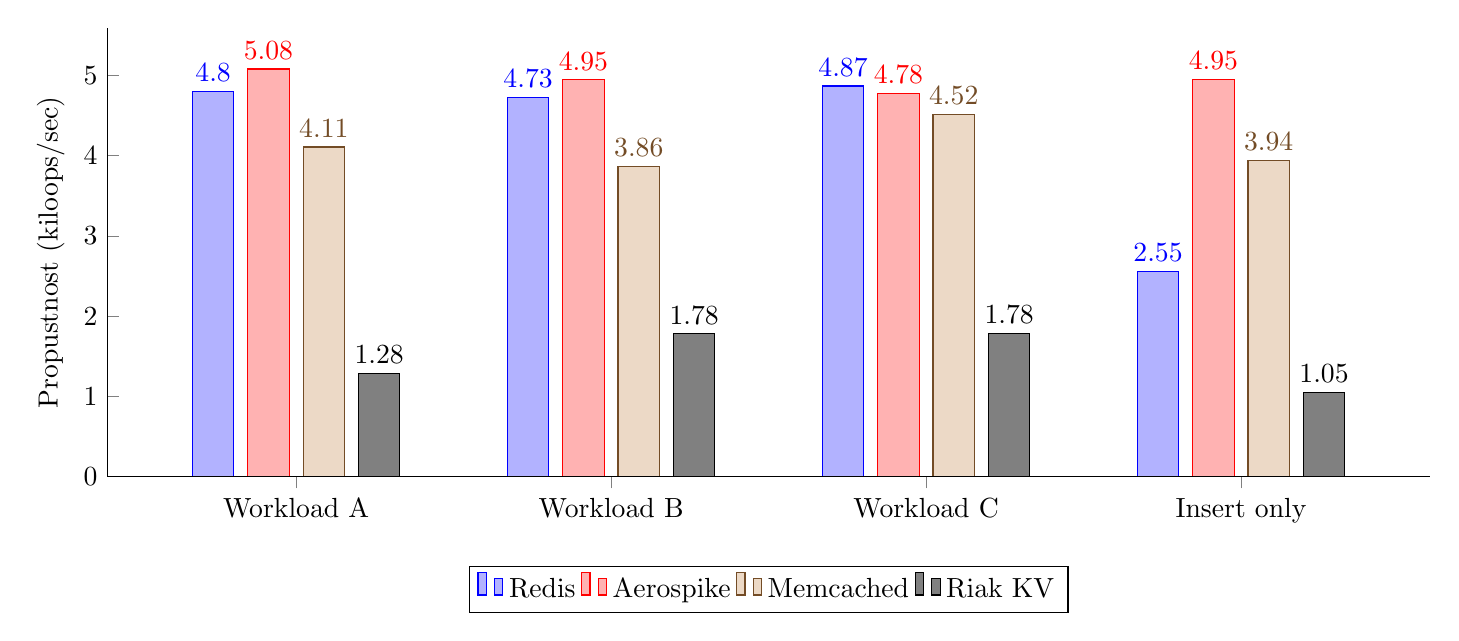
\begin{tikzpicture}
			\begin{axis}[
				ylabel={Propustnost (kiloops/sec)},
				legend style={at={(0.5,-0.2)},
					anchor=north,legend columns=-1},
				every axis plot post/.style={/pgf/number format/fixed},
				ybar=5pt,
				bar width=15pt,
				x=4cm,
				%y=1.5cm,
				ymin=0,
				axis on top,
				%ymax=5.5,
				xtick=data,
				enlarge x limits=0.2,
				symbolic x coords={Workload A, Workload B, Workload C, Insert only},
				%restrict y to domain*=0:6, % Cut values off at 3
				visualization depends on=rawy\as\rawy, % Save the unclipped values
				%after end axis/.code={ % Draw line indicating break
				%	\draw [ultra thick, white, decoration={snake, amplitude=1pt}, decorate] (rel axis cs:0,1.05) -- (rel axis %cs:1,1.05);
				%},
				nodes near coords={%
					\pgfmathprintnumber{\rawy}% Print unclipped values
				},
				axis lines*=left,
				clip=false
				]
				\addplot coordinates {(Workload A,4.8) (Workload B,4.726958) (Workload C,4.8683) (Insert only,2.553)};
				\addplot coordinates {(Workload A,5.081) (Workload B,4.9454377) (Workload C,4.77812) (Insert only,4.95306)};
				\addplot coordinates {(Workload A,4.1087) (Workload B,3.863588) (Workload C,4.51767) (Insert only,3.93796)};
				\addplot coordinates {(Workload A,1.2839777) (Workload B,1.77815) (Workload C,1.7833) (Insert only,1.0524)};
				\legend{Redis,Aerospike,Memcached,Riak KV}
			\end{axis}
		\end{tikzpicture}
		\caption{Workload A, B, C + Insert only - Propustnost (kiloops/sec)}
		\label{graph_Workloads A, B, C + Insert only - Throughput (kiloops/sec)}
	\end{figure}

	\begin{figure}[h]
		\centering
		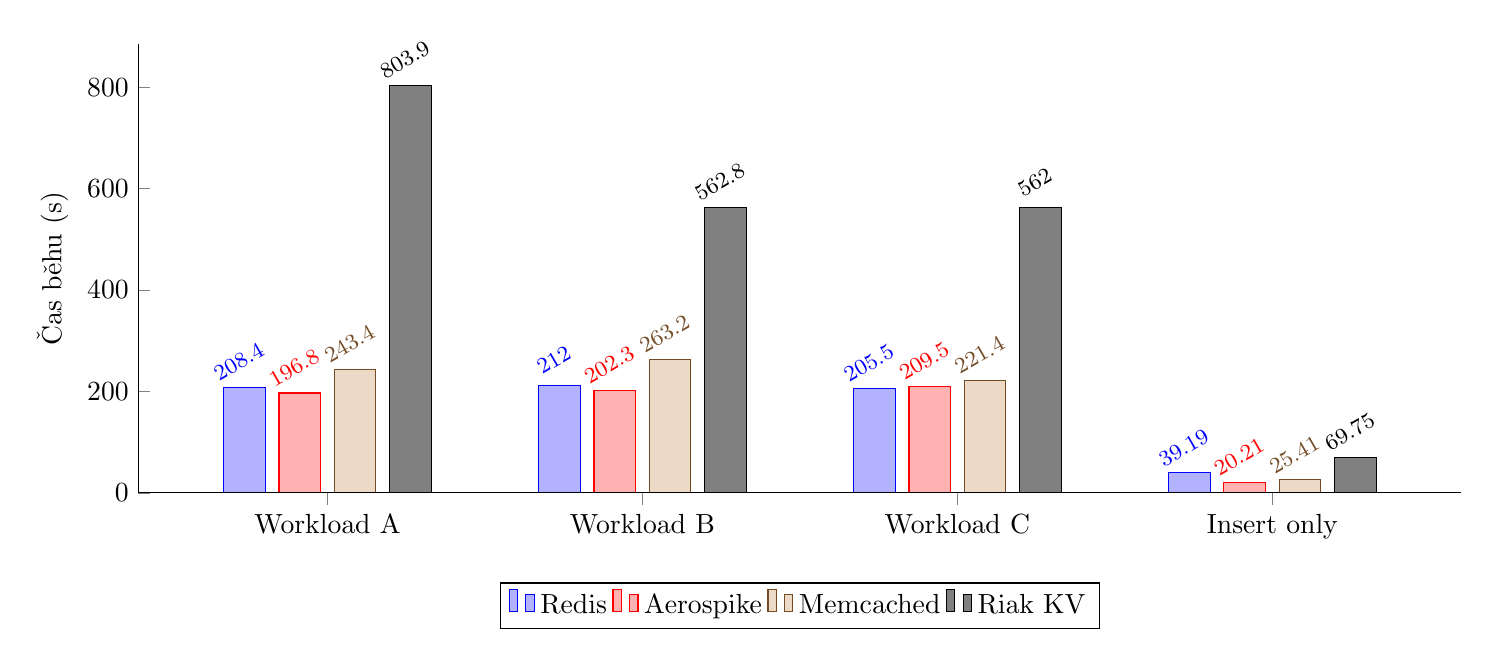
\begin{tikzpicture}
			\begin{axis}[
				ylabel={Čas běhu (s)},
				legend style={at={(0.5,-0.2)}, anchor=north, legend columns=-1},
				every axis plot post/.style={/pgf/number format/fixed},
				ybar=5pt,
				bar width=15pt,
				x=4cm,
				%y=1.5cm, % změněno
				ymin=0,
				axis on top,
				%ymax=500, % změněno
				xtick=data,
				enlarge x limits=0.2,
				symbolic x coords={Workload A, Workload B, Workload C, Insert only},
				%restrict y to domain*=0:6, % Cut values off at 3
				visualization depends on=rawy\as\rawy, % Save the unclipped values
				%after end axis/.code={ % Draw line indicating break
					%    \draw [ultra thick, white, decoration={snake, amplitude=1pt}, decorate] (rel axis cs:0,1.05) -- (rel axis cs:1,1.05);
					%},
				nodes near coords={%
					\pgfmathprintnumber{\rawy}% Print unclipped values
				},
				nodes near coords style={font=\footnotesize, rotate=30, xshift=0.1cm, yshift=0.1cm}, % změněno na north
				%nodes near coords align={left}, % posunuto pouze doleva
				axis lines*=left,
				clip=false,
				]
				\addplot coordinates {(Workload A,208.4) (Workload B,212.0) (Workload C,205.5) (Insert only,39.19)};
				\addplot coordinates {(Workload A,196.8) (Workload B,202.3) (Workload C,209.5) (Insert only,20.21)};
				\addplot coordinates {(Workload A,243.4) (Workload B,263.2) (Workload C,221.4) (Insert only,25.41)};
				\addplot coordinates {(Workload A,803.9) (Workload B,562.8) (Workload C,562.0) (Insert only,69.75)};
				\legend{Redis,Aerospike,Memcached,Riak KV}
			\end{axis}
		\end{tikzpicture}
		\caption{Workload A, B, C + Insert only - Čas běhu (s)}
		\label{graph_Workloads A, B, C + Insert only - Runtime(s)}
	\end{figure}
	
	\begin{figure}[h]
		\centering
		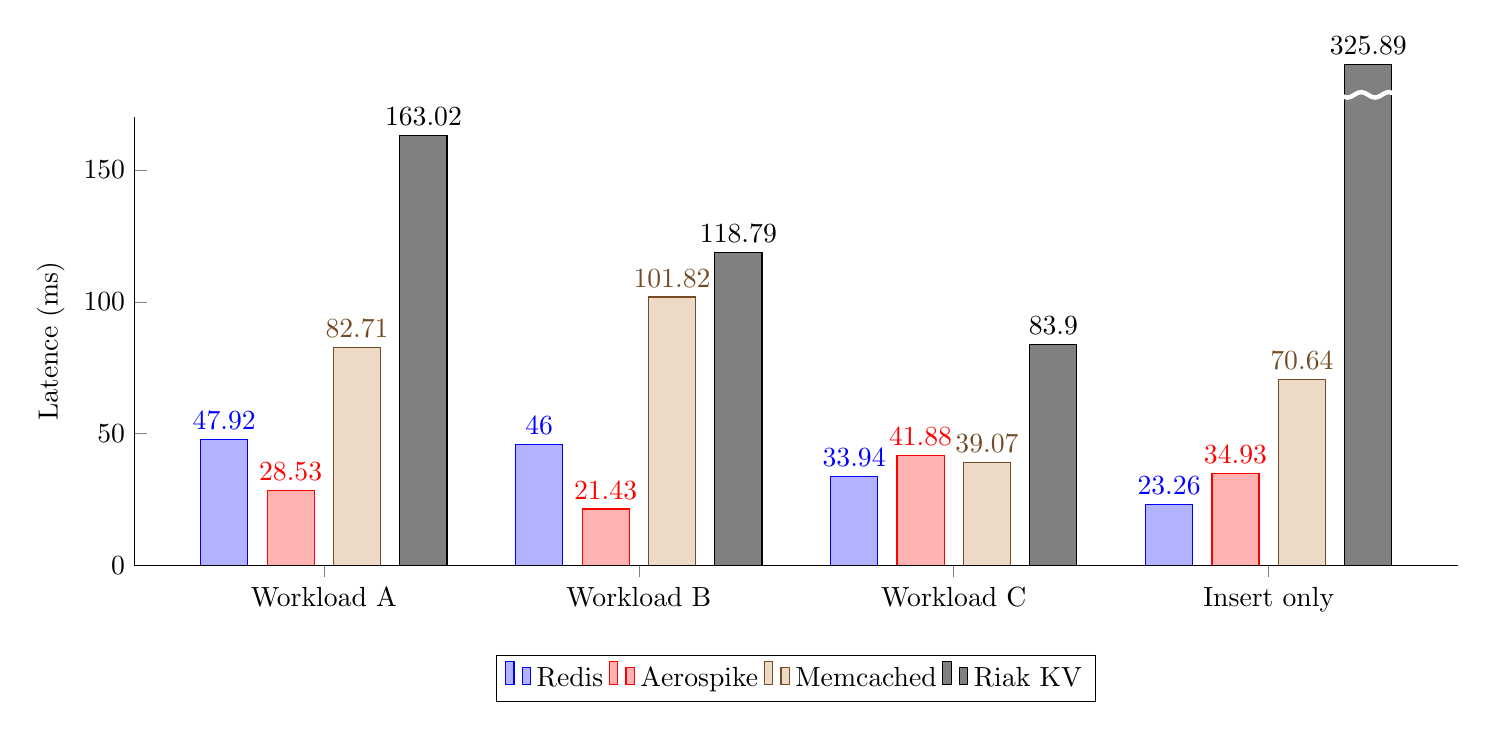
\begin{tikzpicture}
			\begin{axis}[
				ylabel={Latence (ms)},
				legend style={at={(0.5,-0.2)},
					anchor=north,legend columns=-1},
				every axis plot post/.style={/pgf/number format/fixed},
				ybar=7pt,
				bar width=17pt,
				x=4cm,
				%y=1.5cm,
				ymin=0,
				axis on top,
				ymax=170,
				xtick=data,
				enlarge x limits=0.2,
				symbolic x coords={Workload A, Workload B, Workload C, Insert only},
				restrict y to domain*=0:190, % Cut values off at 3
				visualization depends on=rawy\as\rawy, % Save the unclipped values
				after end axis/.code={ % Draw line indicating break
						\draw [ultra thick, white, decoration={snake, amplitude=1pt}, decorate] (rel axis cs:0,1.05) -- (rel axis cs:1,1.05);
				},
				nodes near coords={%
					\pgfmathprintnumber{\rawy}% Print unclipped values
				},
				axis lines*=left,
				clip=false
				]
				\addplot coordinates {(Workload A,47.92) (Workload B,46.00) (Workload C,33.94) (Insert only,23.26)};
				\addplot coordinates {(Workload A,28.53) (Workload B,21.43) (Workload C,41.88) (Insert only,34.93)};
				\addplot coordinates {(Workload A,82.71) (Workload B,101.82) (Workload C,39.07) (Insert only,70.64)};
				\addplot coordinates {(Workload A,163.02) (Workload B,118.79) (Workload C,83.90) (Insert only,325.89)};
				\legend{Redis,Aerospike,Memcached,Riak KV}
			\end{axis}
		\end{tikzpicture}
		\caption{Workload A, B, C + Insert only - Max Latence (ms)}
		\label{graph_Workloads A, B, C + Insert only - Max Latency (ms)}
	\end{figure}
	
	\begin{figure}[h]
		\centering
		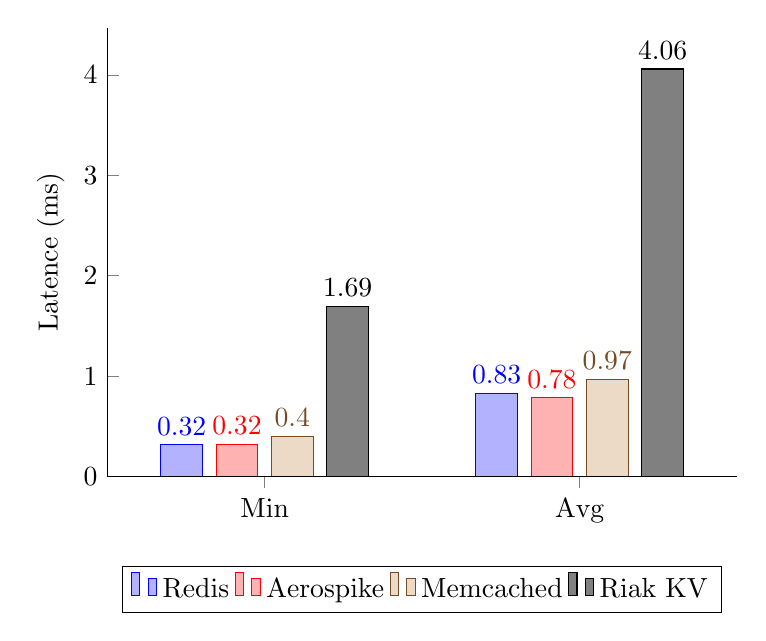
\begin{tikzpicture}
			\begin{axis}[
				ylabel={Latence (ms)},
				symbolic x coords={Min,Avg},
				legend style={at={(0.5,-0.2)},
					anchor=north,legend columns=-1},
				every axis plot post/.style={/pgf/number format/fixed},
				ybar=5pt,
				bar width=15pt,
				x=4cm,
				%xmin=0,
				%width=15cm,
				%y=1.5cm,
				ymin=0,
				axis on top,
				%ymax=200,
				xtick=data,
				%xmin=Min-15,
				%xtick distance=10,
				enlarge x limits=0.5,
				%restrict y to domain*=0:300, % Cut values off at 14
				visualization depends on=rawy\as\rawy, % Save the unclipped values
				%after end axis/.code={ % Draw line indicating break
				%	\draw [ultra thick, white, decoration={snake, amplitude=1pt}, decorate] (rel axis cs:0,1.05) -- (rel axis cs:1,1.05);
				%},
				nodes near coords={%
					\pgfmathprintnumber{\rawy}% Print unclipped values
				},
				axis lines*=left,
				clip=false,
				%extra x ticks={Min, Avg, Max},
				%x tick style={xticklabel style={xshift=-20pt}}
				]
				\addplot coordinates {(Min,0.3151666667) (Avg,0.830447166)};
				\addplot coordinates {(Min,0.317) (Avg,0.7842715474)};
				\addplot coordinates {(Min,0.4015) (Avg,0.9679028534)};
				\addplot coordinates {(Min,1.694) (Avg,4.058593436)};
				\legend{Redis,Aerospike,Memcached,Riak KV}
			\end{axis}
		\end{tikzpicture}
		\caption{Workload A - Min Avg Latence (ms)}
		\label{graph_Workload A - Min Avg Latency (ms)}
	\end{figure}
	
	\begin{figure}[h]
		\centering
		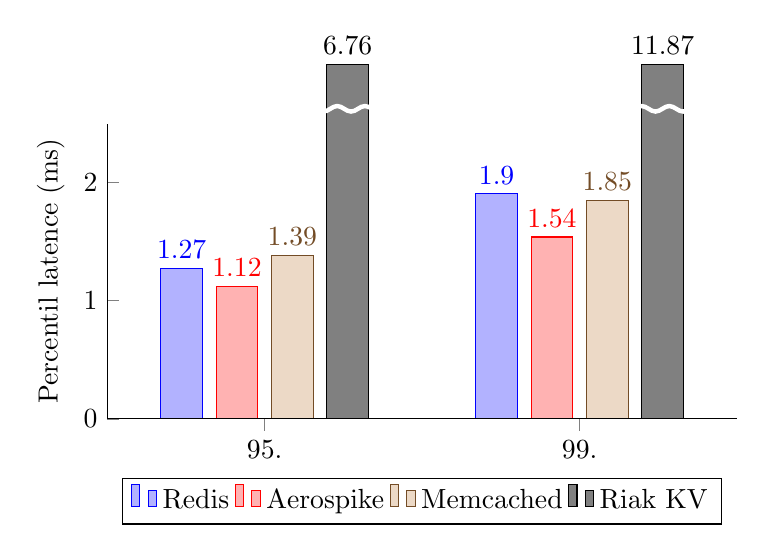
\begin{tikzpicture}
			\begin{axis}[
				ylabel={Percentil latence (ms)},
				legend style={at={(0.5,-0.2)},
					anchor=north,legend columns=-1},
				every axis plot post/.style={/pgf/number format/fixed},
				ybar=5pt,
				bar width=15pt,
				x=4cm,
				y=1.5cm,
				ymin=0,
				axis on top,
				ymax=2.5,
				xtick=data,
				enlarge x limits=0.5,
				symbolic x coords={95.,99.},
				restrict y to domain*=0:3, % Cut values off at 14
				visualization depends on=rawy\as\rawy, % Save the unclipped values
				after end axis/.code={ % Draw line indicating break
					\draw [ultra thick, white, decoration={snake, amplitude=1pt}, decorate] (rel axis cs:0,1.05) -- (rel axis cs:1,1.05);
				},
				nodes near coords={%
					\pgfmathprintnumber{\rawy}% Print unclipped values
				},
				axis lines*=left,
				clip=false
				]
				\addplot coordinates {(95.,1.273) (99.,1.9045)};
				\addplot coordinates {(95.,1.12183) (99.,1.5393)};
				\addplot coordinates {(95.,1.3863) (99.,1.8483)};
				\addplot coordinates {(95.,6.757) (99.,11.8656)};
				\legend{Redis,Aerospike,Memcached,Riak KV}
			\end{axis}
		\end{tikzpicture}
		\caption{Workload A - Percentil latence (ms)}
		\label{graph_Workload A - Percentile Latency (ms)}
	\end{figure}

	\begin{figure}[h]
		\centering
		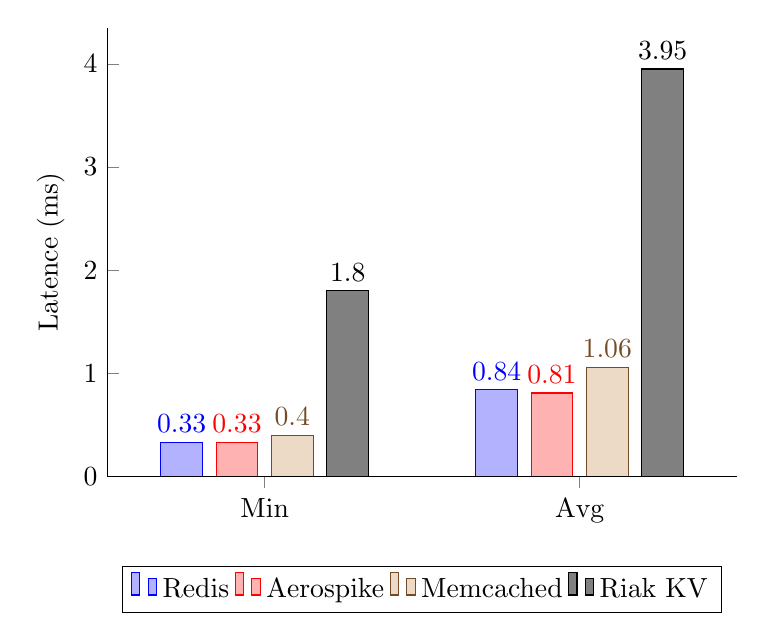
\begin{tikzpicture}
			\begin{axis}[
				ylabel={Latence (ms)},
				symbolic x coords={Min,Avg},
				legend style={at={(0.5,-0.2)},
					anchor=north,legend columns=-1},
				every axis plot post/.style={/pgf/number format/fixed},
				ybar=5pt,
				bar width=15pt,
				x=4cm,
				%xmin=0,
				%width=15cm,
				%y=1.5cm,
				ymin=0,
				axis on top,
				%ymax=200,
				xtick=data,
				%xmin=Min-15,
				%xtick distance=10,
				enlarge x limits=0.5,
				%restrict y to domain*=0:300, % Cut values off at 14
				visualization depends on=rawy\as\rawy, % Save the unclipped values
				%after end axis/.code={ % Draw line indicating break
					%	\draw [ultra thick, white, decoration={snake, amplitude=1pt}, decorate] (rel axis cs:0,1.05) -- (rel axis cs:1,1.05);
					%},
				nodes near coords={%
					\pgfmathprintnumber{\rawy}% Print unclipped values
				},
				axis lines*=left,
				clip=false,
				%extra x ticks={Min, Avg, Max},
				%x tick style={xticklabel style={xshift=-20pt}}
				]
				\addplot coordinates {(Min,0.33) (Avg,0.84)};
				\addplot coordinates {(Min,0.33) (Avg,0.81)};
				\addplot coordinates {(Min,0.40) (Avg,1.06)};
				\addplot coordinates {(Min,1.80) (Avg,3.95)};
				\legend{Redis,Aerospike,Memcached,Riak KV}
			\end{axis}
		\end{tikzpicture}
		\caption{Workload B - Min Avg Latence (ms)}
		\label{graph_Workload B - Min Avg Latency (ms)}
	\end{figure}

	\begin{figure}[h]
		\centering
		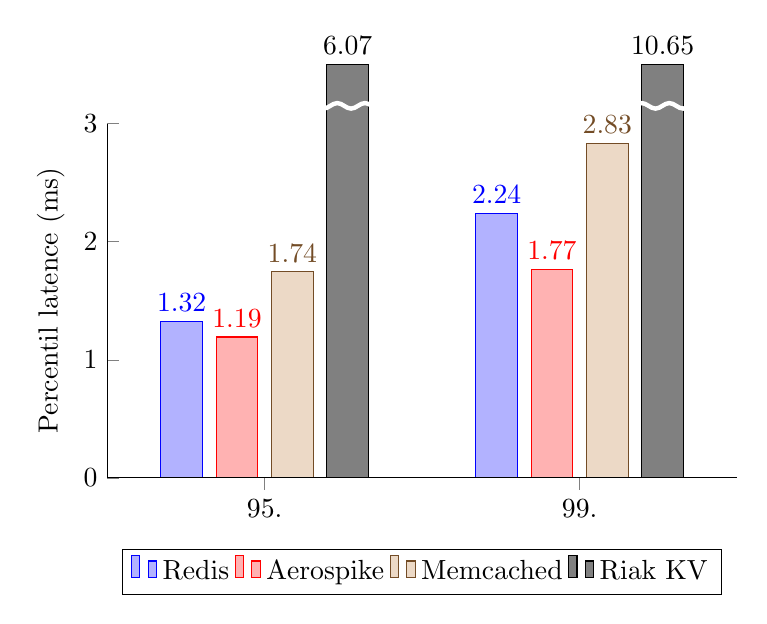
\begin{tikzpicture}
			\begin{axis}[
				ylabel={Percentil latence (ms)},
				legend style={at={(0.5,-0.2)},
					anchor=north,legend columns=-1},
				every axis plot post/.style={/pgf/number format/fixed},
				ybar=5pt,
				bar width=15pt,
				x=4cm,
				y=1.5cm,
				ymin=0,
				axis on top,
				ymax=3,
				xtick=data,
				enlarge x limits=0.5,
				symbolic x coords={95.,99.},
				restrict y to domain*=0:3.5, % Cut values off at 3
				visualization depends on=rawy\as\rawy, % Save the unclipped values
				after end axis/.code={ % Draw line indicating break
					\draw [ultra thick, white, decoration={snake, amplitude=1pt}, decorate] (rel axis cs:0,1.05) -- (rel axis cs:1,1.05);
				},
				nodes near coords={%
					\pgfmathprintnumber{\rawy}% Print unclipped values
				},
				axis lines*=left,
				clip=false
				]
				\addplot coordinates {(95.,1.3236) (99.,2.237833)};
				\addplot coordinates {(95.,1.19283) (99.,1.76783)};
				\addplot coordinates {(95.,1.744) (99.,2.832)};
				\addplot coordinates {(95.,6.06766) (99.,10.65033)};
				\legend{Redis,Aerospike,Memcached,Riak KV}
			\end{axis}
		\end{tikzpicture}
		\caption{Workload B - Percentil latence (ms)}
		\label{graph_Workload B - Percentile Latency (ms)}
	\end{figure}

	\begin{figure}[h]
		\centering
		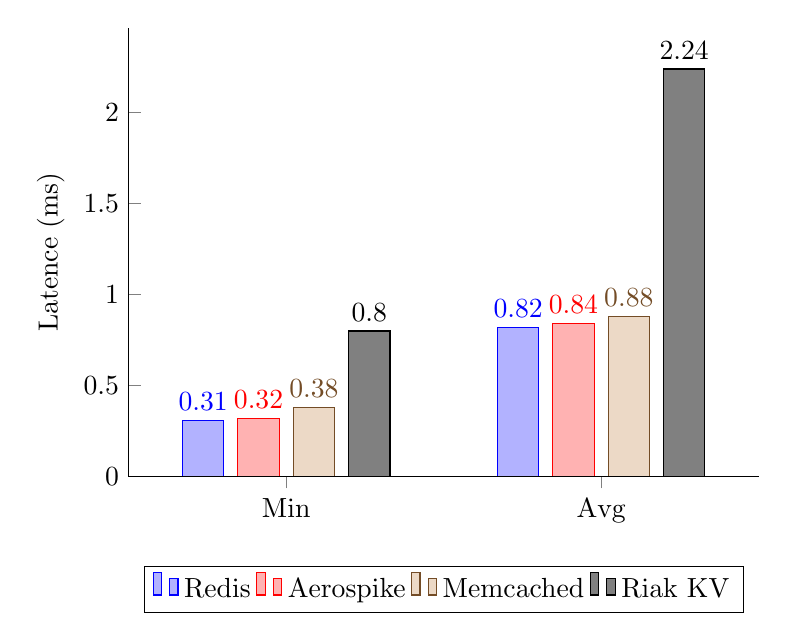
\begin{tikzpicture}
			\begin{axis}[
				ylabel={Latence (ms)},
				symbolic x coords={Min,Avg},
				legend style={at={(0.5,-0.2)},
					anchor=north,legend columns=-1},
				every axis plot post/.style={/pgf/number format/fixed},
				ybar=5pt,
				bar width=15pt,
				x=4cm,
				%xmin=0,
				%width=15cm,
				%y=1.5cm,
				ymin=0,
				axis on top,
				%ymax=200,
				xtick=data,
				%xmin=Min-15,
				%xtick distance=10,
				enlarge x limits=0.5,
				%restrict y to domain*=0:300, % Cut values off at 14
				visualization depends on=rawy\as\rawy, % Save the unclipped values
				%after end axis/.code={ % Draw line indicating break
					%	\draw [ultra thick, white, decoration={snake, amplitude=1pt}, decorate] (rel axis cs:0,1.05) -- (rel axis cs:1,1.05);
					%},
				nodes near coords={%
					\pgfmathprintnumber{\rawy}% Print unclipped values
				},
				axis lines*=left,
				clip=false,
				%extra x ticks={Min, Avg, Max},
				%x tick style={xticklabel style={xshift=-20pt}}
				]
				\addplot coordinates {(Min,0.31) (Avg,0.82)};
				\addplot coordinates {(Min,0.32) (Avg,0.84)};
				\addplot coordinates {(Min,0.38) (Avg,0.88)};
				\addplot coordinates {(Min,0.80) (Avg,2.24)};
				\legend{Redis,Aerospike,Memcached,Riak KV}
			\end{axis}
		\end{tikzpicture}
		\caption{Workload C - Min Avg Latence (ms)}
		\label{graph_Workload C - Min Avg Latency (ms)}
	\end{figure}

	\begin{figure}[h]
		\centering
		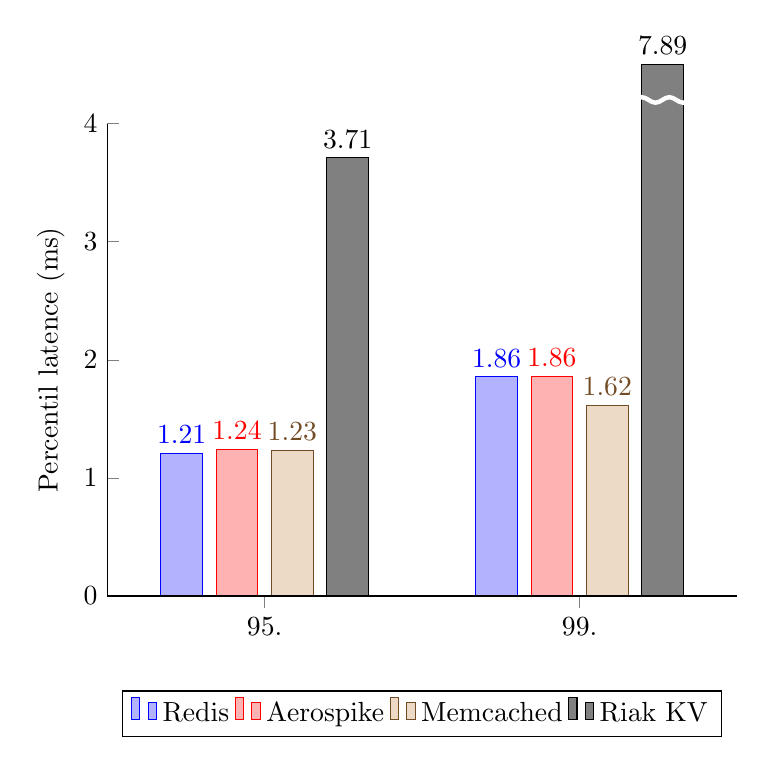
\begin{tikzpicture}
			\begin{axis}[
				ylabel={Percentil latence (ms)},
				legend style={at={(0.5,-0.2)},
					anchor=north,legend columns=-1},
				every axis plot post/.style={/pgf/number format/fixed},
				ybar=5pt,
				bar width=15pt,
				x=4cm,
				y=1.5cm,
				ymin=0,
				axis on top,
				ymax=4,
				xtick=data,
				enlarge x limits=0.5,
				symbolic x coords={95.,99.},
				restrict y to domain*=0:4.5, % Cut values off at 3
				visualization depends on=rawy\as\rawy, % Save the unclipped values
				after end axis/.code={ % Draw line indicating break
					\draw [ultra thick, white, decoration={snake, amplitude=1pt}, decorate] (rel axis cs:0,1.05) -- (rel axis cs:1,1.05);
				},
				nodes near coords={%
					\pgfmathprintnumber{\rawy}% Print unclipped values
				},
				axis lines*=left,
				clip=false
				]
				\addplot coordinates {(95.,1.21) (99.,1.856)};
				\addplot coordinates {(95.,1.24) (99.,1.8616)};
				\addplot coordinates {(95.,1.23) (99.,1.6153)};
				\addplot coordinates {(95.,3.71) (99.,7.8856)};
				\legend{Redis,Aerospike,Memcached,Riak KV}
			\end{axis}
		\end{tikzpicture}
		\caption{Workload C - Percentil latence (ms)}
		\label{graph_Workload C - Percentile Latency (ms)}
	\end{figure}
	
	\begin{figure}[h]
		\centering
		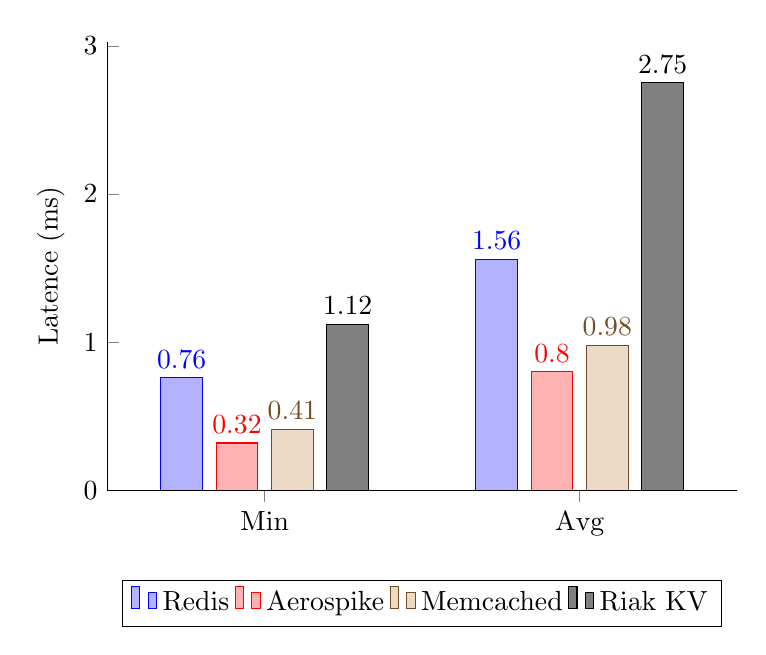
\begin{tikzpicture}
			\begin{axis}[
				ylabel={Latence (ms)},
				symbolic x coords={Min,Avg},
				legend style={at={(0.5,-0.2)},
					anchor=north,legend columns=-1},
				every axis plot post/.style={/pgf/number format/fixed},
				ybar=5pt,
				bar width=15pt,
				x=4cm,
				%xmin=0,
				%width=15cm,
				%y=1.5cm,
				ymin=0,
				axis on top,
				%ymax=200,
				xtick=data,
				%xmin=Min-15,
				%xtick distance=10,
				enlarge x limits=0.5,
				%restrict y to domain*=0:300, % Cut values off at 14
				visualization depends on=rawy\as\rawy, % Save the unclipped values
				%after end axis/.code={ % Draw line indicating break
					%	\draw [ultra thick, white, decoration={snake, amplitude=1pt}, decorate] (rel axis cs:0,1.05) -- (rel axis cs:1,1.05);
					%},
				nodes near coords={%
					\pgfmathprintnumber{\rawy}% Print unclipped values
				},
				axis lines*=left,
				clip=false,
				%extra x ticks={Min, Avg, Max},
				%x tick style={xticklabel style={xshift=-20pt}}
				]
				\addplot coordinates {(Min,0.76) (Avg,1.56)};
				\addplot coordinates {(Min,0.32) (Avg,0.80)};
				\addplot coordinates {(Min,0.41) (Avg,0.98)};
				\addplot coordinates {(Min,1.12) (Avg,2.75)};
				\legend{Redis,Aerospike,Memcached,Riak KV}
			\end{axis}
		\end{tikzpicture}
		\caption{Insert only - Min Avg Latence (ms)}
		\label{graph_Insert only - Min Avg Latency (ms)}
	\end{figure}
	
	\begin{figure}[h]
		\centering
		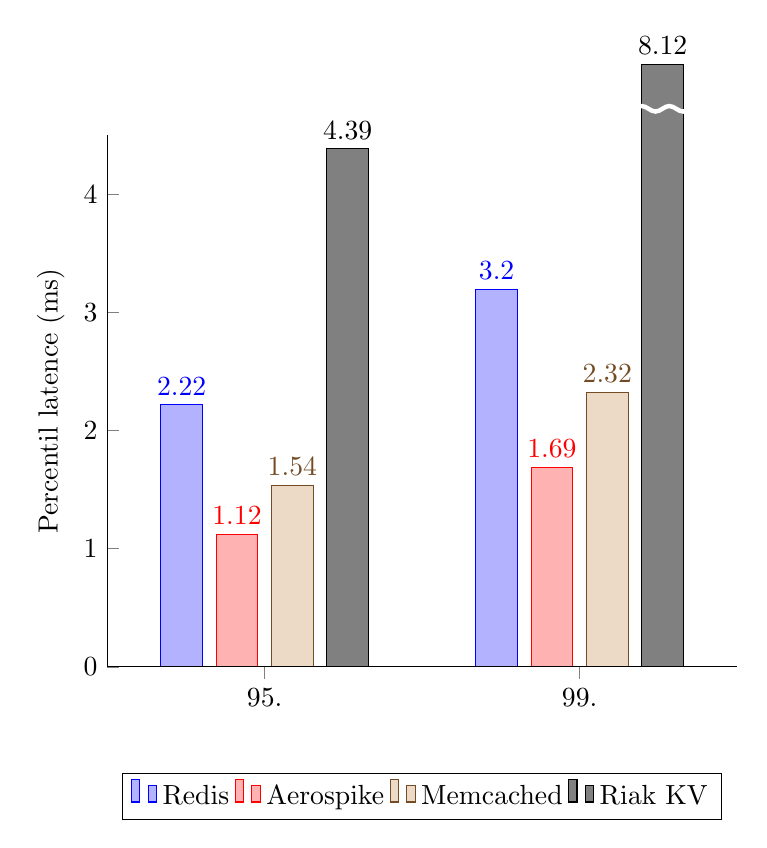
\begin{tikzpicture}
			\begin{axis}[
				ylabel={Percentil latence (ms)},
				legend style={at={(0.5,-0.2)},
					anchor=north,legend columns=-1},
				every axis plot post/.style={/pgf/number format/fixed},
				ybar=5pt,
				bar width=15pt,
				x=4cm,
				y=1.5cm,
				ymin=0,
				axis on top,
				ymax=4.5,
				xtick=data,
				enlarge x limits=0.5,
				symbolic x coords={95.,99.},
				restrict y to domain*=0:5.1, % Cut values off at 3
				visualization depends on=rawy\as\rawy, % Save the unclipped values
				after end axis/.code={ % Draw line indicating break
					\draw [ultra thick, white, decoration={snake, amplitude=1pt}, decorate] (rel axis cs:0,1.05) -- (rel axis cs:1,1.05);
				},
				nodes near coords={%
					\pgfmathprintnumber{\rawy}% Print unclipped values
				},
				axis lines*=left,
				clip=false
				]
				\addplot coordinates {(95.,2.219) (99.,3.195)};
				\addplot coordinates {(95.,1.11933) (99.,1.690)};
				\addplot coordinates {(95.,1.5366) (99.,2.32233)};
				\addplot coordinates {(95.,4.3863) (99.,8.12433)};
				\legend{Redis,Aerospike,Memcached,Riak KV}
			\end{axis}
		\end{tikzpicture}
		\caption{Insert only - Percentil latence (ms)}
		\label{graph_Insert only - Percentile Latency (ms)}
	\end{figure}
	
	\chapter{Závěr\label{chapter:5-diploma_results}}
	
	TODO
		
	\nocite{*}
	
	\printbibliography[title={Literatura}, heading=bibintoc]
	
\end{document}